\documentclass[conference]{IEEEtran}

\usepackage{cite}
\usepackage{url}
\usepackage{listings}
\usepackage{courier}
\lstset{
basicstyle=\footnotesize\ttfamily,
breaklines=true,
breakatwhitespace=true,
columns=fullflexible
}
\usepackage{graphicx}
\usepackage{amsmath}
\usepackage{xcolor}
\usepackage{float}
\usepackage{hyperref}



\title{
Investigating and Implementing LibreRouter and LibreMesh:
Virtualized and Raspberry Pi-Based Mesh Networking
}

\author{
\IEEEauthorblockN{\small
Bastas, Dimitrios (LT),
Kamilos, Dimitrios (LT)\\
Rachel Goldstein (LT),
Robert Leyba (LT)\\
Margaret Moore (LTJG)
}
\IEEEauthorblockA{
EC3730 Final Project
}
}

\begin{document}

\maketitle

\begin{abstract}

This project investigates LibreRouter and LibreMesh, open-source community networking technologies built on top of OpenWrt. A virtualized OpenWrt environment was developed using VMware Workstation Pro to simulate a four-node routed mesh backbone topology for distributed routing and mesh-network experimentation.

Due to wireless hardware requirements within LibreMesh, OpenWrt with BATMAN-adv was utilized in a virtual environment to emulate and evaluate the same characteristics. 

The project will later extend the deployment onto Raspberry Pi hardware platforms for physical mesh networking experimentation and wireless performance evaluation.

\end{abstract}

\section{Introduction}

Community mesh networks provide decentralized communication infrastructure capable of operating independently of centralized Internet Service Providers (ISPs). LibreRouter and LibreMesh were developed to support resilient, community-owned wireless infrastructure using open-source software and commodity hardware.

This project investigates LibreMesh deployment using both virtualized and physical implementations. Primary goals include evaluating routing behavior, deployment complexity, resilience, security considerations, and operational limitations associated with decentralized mesh infrastructure.

In addition to traditional research analysis, this report maintains a reproducible engineering notebook style documenting implementation steps, troubleshooting observations, operational anomalies, and experimental outcomes throughout the project lifecycle.

\section{Background Research}

\subsection{OpenWrt}

OpenWrt is an open-source Linux-based operating system designed for embedded networking devices such as routers and access points. Unlike traditional vendor firmware, OpenWrt provides a writable filesystem, modular package management, and extensive routing customization capabilities.

In addition to embedded hardware deployments, OpenWrt supports x86 virtualized environments, making it suitable for experimental mesh-networking research.

\subsection{LibreMesh}

LibreMesh is a framework built on top of OpenWrt that simplifies decentralized mesh-network deployment. The platform automates wireless mesh configuration while supporting routing protocols such as BATMAN-adv and BMX7.

LibreMesh was designed for community-operated networks in which nodes dynamically discover neighboring devices and establish resilient communication paths without centralized infrastructure.

LibreMesh includes a feature known as AnyGW (Any Gateway), which allows nodes with Internet connectivity to advertise themselves as gateways to the rest of the mesh network. Client devices use a shared virtual gateway address, while the mesh automatically selects an appropriate Internet-connected node to forward traffic toward external networks. This approach enables Internet access to be distributed throughout the mesh without requiring manual gateway configuration on each node. AnyGW improves scalability and resilience by allowing gateway services to be dynamically discovered and utilized as network conditions change. \cite{libremesh_anygw,libremesh_howitworks}

\subsection{LibreRouter}

LibreRouter is an open-hardware networking platform developed specifically for community mesh deployments. The platform combines OpenWrt-based firmware with wireless hardware optimized for long-range and community-managed networking applications.

\section{Literature Review and Security Analysis}

\subsection{LibreMesh and LibreRouter Deployment Model}

LibreMesh is described as a modular framework for creating OpenWrt-based firmware images for wireless mesh nodes. Its goal is to simplify community mesh-network deployment by automating configuration that would otherwise require significant manual OpenWrt networking knowledge \cite{libremeshdocs}. LibreMesh packages support automatic configuration of mesh behavior, while LibreRouter represents a hardware platform designed specifically for community wireless mesh networks \cite{limerouteredt}.

The LibreMesh getting-started documentation recommends hardware with at least 16 MB of flash, 128 MB of RAM, one operational 2.4 GHz radio, and one operational 5 GHz radio \cite{libremeshgettingstarted}. This hardware requirement is significant because VMware virtual machines emulate Ethernet interfaces rather than true IEEE 802.11 wireless radios. As a result, this project could validate BATMAN-adv mesh behavior over virtual Ethernet, but not full RF-based LibreMesh wireless operation.

\subsection{BATMAN-adv Routing Literature}

BATMAN-adv is a Linux kernel-based Layer 2 mesh routing protocol. Unlike traditional Layer 3 routing protocols, BATMAN-adv forwards Ethernet frames and presents participating mesh nodes as if they were connected through a distributed virtual switch \cite{batmanadvdocs}. OpenWrt documentation identifies batman-adv as the recommended modern BATMAN implementation for local mesh deployments \cite{openwrtbatman}.

BATMAN-adv uses originator messages and distributed topology information to select forwarding paths dynamically. LibreMesh documentation notes that BATMAN-adv periodically sends Originator Messages, with protocol timing affecting convergence speed and control traffic overhead \cite{libremeshprotocols}. This aligns with the experimental observations in this project, where node failure, recovery, and reintegration were visible through BATMAN neighbor and originator tables.

\subsection{Community Network Case Studies}

Community mesh networks have been studied and deployed in multiple real-world environments. Guifi.net is one of the most widely cited examples of a large-scale community network. Research on Guifi.net describes a crowdsourced network infrastructure operated as a shared commons and supported by community-developed tools and governance processes \cite{guifinetcommons}. Additional experimental analysis of Guifi.net evaluated wireless community mesh behavior and highlighted the operational complexity of hybrid wired and wireless links \cite{guifinetexperimental}.

Freifunk provides another major example of community mesh networking. The Gluon firmware framework, used by multiple Freifunk communities, is also based on OpenWrt and provides modular firmware generation for wireless mesh nodes \cite{gluon}. This parallels LibreMesh by showing that community networks often require repeatable firmware-building tools rather than one-off manual router configuration.

NYC Mesh provides a U.S.-based example of volunteer-operated community networking. NYC Mesh uses rooftop wireless links and community-operated infrastructure to provide local broadband access, demonstrating that mesh and community-network concepts can scale beyond laboratory environments \cite{nycmeshcase}. These case studies show that the technical challenges encountered in this project, including addressing, routing, management, and hardware constraints, are also present in real community-network deployments.

\subsection{Security Weaknesses and Operational Risks}

Wireless mesh networks introduce several security and operational risks. General wireless mesh security literature identifies attacks involving unauthorized access, routing disruption, malicious node participation, denial-of-service, and traffic interception \cite{wmnsecurity}. Because mesh networks rely on peer participation and distributed forwarding, compromised or misconfigured nodes can affect more than one local link.

OpenWrt package management and update behavior also represent an important security area. OpenWrt security documentation notes that user-space packages can be updated relatively quickly, while kernel and kernel-module fixes may require new releases \cite{openwrtsecurity}. This is relevant because BATMAN-adv depends on kernel-module support, and kernel-module availability affects whether mesh routing can be deployed or patched easily.

The project also encountered package-management weaknesses during implementation. BusyBox wget lacked HTTPS support in the tested OpenWrt image, forcing temporary downgrade from HTTPS to HTTP repository access. This introduced potential risks including repository spoofing, package tampering, and man-in-the-middle attacks. OpenWrt package-signature issues have also appeared in public issue reports, demonstrating that repository trust and update-chain reliability are practical concerns rather than purely theoretical risks \cite{openwrtsigissue}.

\subsection{Implementation Lessons from Prior Projects}

Prior mesh projects demonstrate that deployment repeatability is essential. LibreMesh, Gluon, and OpenWrt ImageBuilder workflows all emphasize firmware generation, package selection, and hardware compatibility. This supports the need for exported configuration files and repeatable setup scripts in this project.

The Commotion project provides another example of decentralized mesh-network tooling and emphasizes usability, configuration management, and security review in mesh-network deployments \cite{commotionaudit}. These lessons align with this project's experience: successful routing was only one part of the deployment; management access, configuration persistence, file transfer, script compatibility, and reproducible exports were also required to create a usable mesh-network testbed.

\subsection{Summary of Identified Weaknesses}

The literature review and project implementation identified several major weakness categories:

\begin{itemize}
    \item Hardware dependency on supported wireless radios for full LibreMesh deployment
    \item Package-management and update-chain risks in embedded router systems
    \item Kernel-module dependency for BATMAN-adv functionality
    \item Potential routing disruption from malicious or misconfigured mesh nodes
    \item Management-plane instability caused by cloned router identities and DHCP conflicts
    \item IPv6 duplicate-address behavior after virtual-machine cloning
    \item Limited realism of virtual Ethernet compared to physical wireless RF environments
    \item Need for repeatable configuration export and deployment documentation
\end{itemize}

\section{Virtualized OpenWrt Deployment}

\subsection{Virtualization Environment}

VMware Workstation Pro 17 was selected as the virtualization platform for the initial implementation phase. Virtualization provided rapid deployment, rollback capability through snapshots, reproducible experimentation, and simplified troubleshooting prior to deployment on physical Raspberry Pi hardware.

\subsection{OpenWrt Image Preparation}

The OpenWrt x86\_64 ext4 combined image was downloaded from the official OpenWrt release repository. Since VMware does not natively boot raw IMG files efficiently, the OpenWrt disk image was converted into VMware VMDK format prior to deployment.

\subsection{Virtual Machine Configuration}

A custom virtual machine configuration was selected in VMware Workstation Pro to allow manual control over networking interfaces and storage configuration.

\begin{table}[H]
\centering
\caption{Initial OpenWrt VM Configuration}
\begin{tabular}{|l|l|}
\hline
Setting & Value \\ \hline
Guest OS & Other Linux 5.x 64-bit \\ \hline
vCPUs & 1 \\ \hline
Memory & 256 MB \\ \hline
Primary Disk & OpenWrt VMDK \\ \hline
Network Adapter 1 & NAT \\ \hline
Network Adapter 2 & Host-only \\ \hline
\end{tabular}
\end{table}

\subsection{Network Interface Design}

Two virtual network adapters were configured for each virtual router node:

\begin{itemize}
    \item NAT adapter for WAN connectivity and package installation
    \item Host-only adapter for internal mesh backbone communication
\end{itemize}

This architecture allowed the virtual environment to simulate isolated routed mesh connectivity while preserving Internet access for package installation and updates.

\subsection{Initial Boot Validation}

The OpenWrt virtual machine booted successfully after the VMDK disk image was attached to the VMware virtual SCSI controller.

During startup, OpenWrt initialized both virtual Ethernet interfaces successfully:

\begin{lstlisting}
eth0 NIC Link is Up
eth1 NIC Link is Up
\end{lstlisting}

The successful initialization confirmed that VMware virtual networking devices were correctly recognized by the OpenWrt kernel.

\begin{figure}[H]
\centering
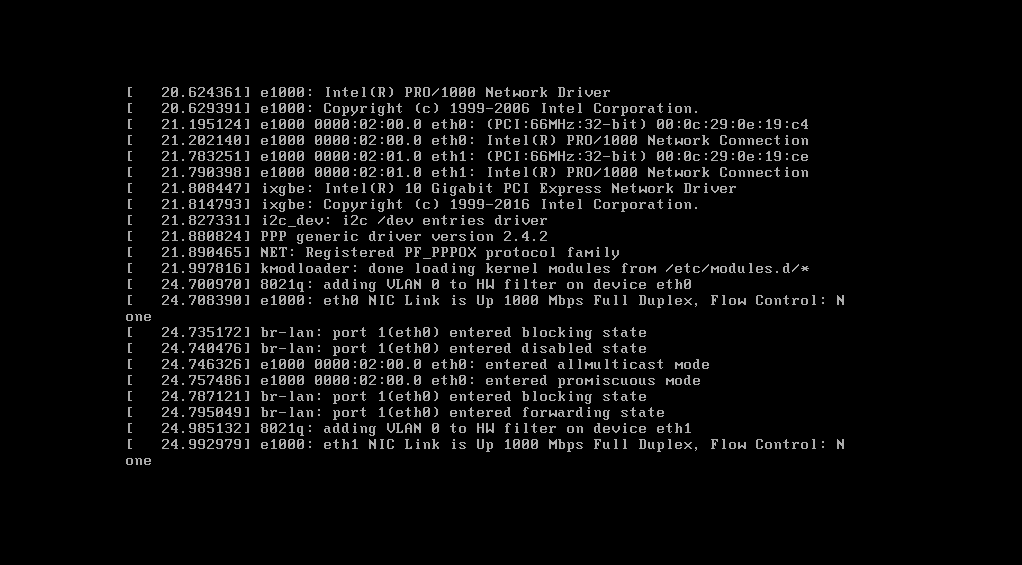
\includegraphics[width=0.45\textwidth]{figures/openwrt-first-init.png}
\caption{Successful OpenWrt boot and interface initialization.}
\label{fig:bootlog}
\end{figure}

\section{Network Troubleshooting and Recovery}

\subsection{Initial Connectivity Failure}

Initial deployment attempts failed to provide Internet connectivity.

Observed symptoms included:

\begin{itemize}
    \item Missing default routes
    \item Failed DNS resolution
    \item Inability to ping external IP addresses
    \item DHCP inconsistencies
\end{itemize}

Example failure:

\begin{lstlisting}
ping -c 4 8.8.8.8
Network unreachable
\end{lstlisting}

Investigation revealed that VMware host-only networking was unintentionally acting as the WAN DHCP source, creating interface ambiguity and routing instability.

Observed VMware virtual networks included:

\begin{itemize}
    \item VMnet1: 192.168.61.0/24
    \item VMnet8: 192.168.111.0/24
\end{itemize}

\subsection{Controlled Simplification Strategy}

To isolate the networking issue, the second adapter was temporarily removed and the deployment simplified to a single NAT interface.

After simplification, the OpenWrt node successfully received:

\begin{itemize}
    \item DHCP assignment
    \item Default gateway
    \item External DNS access
\end{itemize}

Working configuration:

\begin{lstlisting}
default via 192.168.111.2 dev eth0
\end{lstlisting}

Successful validation tests included:

\begin{lstlisting}
ping -c 4 8.8.8.8
ping -c 4 google.com
\end{lstlisting}

All tests completed successfully with zero packet loss.

\subsection{Package Management Failure Analysis}

Package management operations initially failed during APK repository access.

Observed errors included:

\begin{lstlisting}
wget exited with error 1
unexpected end of file
\end{lstlisting}

Further investigation revealed that BusyBox wget lacked HTTPS support:

\begin{lstlisting}
wget https://downloads.openwrt.org/
HTTPS support not compiled in.
\end{lstlisting}

This explained repeated failures retrieving APK repository metadata over HTTPS and forced temporary downgrade of repository transport from HTTPS to HTTP in order to restore package functionality.

Potential security implications included:

\begin{itemize}
    \item Man-in-the-middle attacks
    \item Package tampering
    \item Repository spoofing
    \item Supply-chain compromise
\end{itemize}

\subsection{Temporary Package Recovery}

HTTPS functionality was partially restored by manually transferring APK packages into the virtual machine and installing them locally:

\begin{lstlisting}
apk add --allow-untrusted ./*.apk
\end{lstlisting}

Repository transport was later temporarily modified from HTTPS to HTTP to restore repository index access.

After modification:

\begin{lstlisting}
apk update
\end{lstlisting}

successfully completed.

Core administrative packages were then installed successfully:

\begin{lstlisting}
apk add nano
apk add vim
apk add curl
apk add tcpdump
apk add htop
apk add bash
apk add luci
\end{lstlisting}

\section{LuCI Web Interface Deployment}

After installation of LuCI, the OpenWrt web interface was initially inaccessible through:

\begin{lstlisting}
http://192.168.1.1
\end{lstlisting}

Diagnostic analysis using:

\begin{lstlisting}
netstat -tlnp
\end{lstlisting}

confirmed that the web server was actively listening on ports 80 and 443:

\begin{lstlisting}
0.0.0.0:80 LISTEN
0.0.0.0:443 LISTEN
\end{lstlisting}

Further analysis revealed that the Windows host system could directly access only the VMware NAT interface rather than the internal OpenWrt LAN bridge. As a result, the LuCI interface became accessible using:

\begin{lstlisting}
http://192.168.111.130
\end{lstlisting}

rather than the internal bridge address.

This demonstrated the distinction between:

\begin{itemize}
    \item Internal OpenWrt LAN addressing
    \item Externally reachable VMware NAT addressing
    \item Hypervisor network segmentation behavior
\end{itemize}

\begin{figure}[H]
\centering
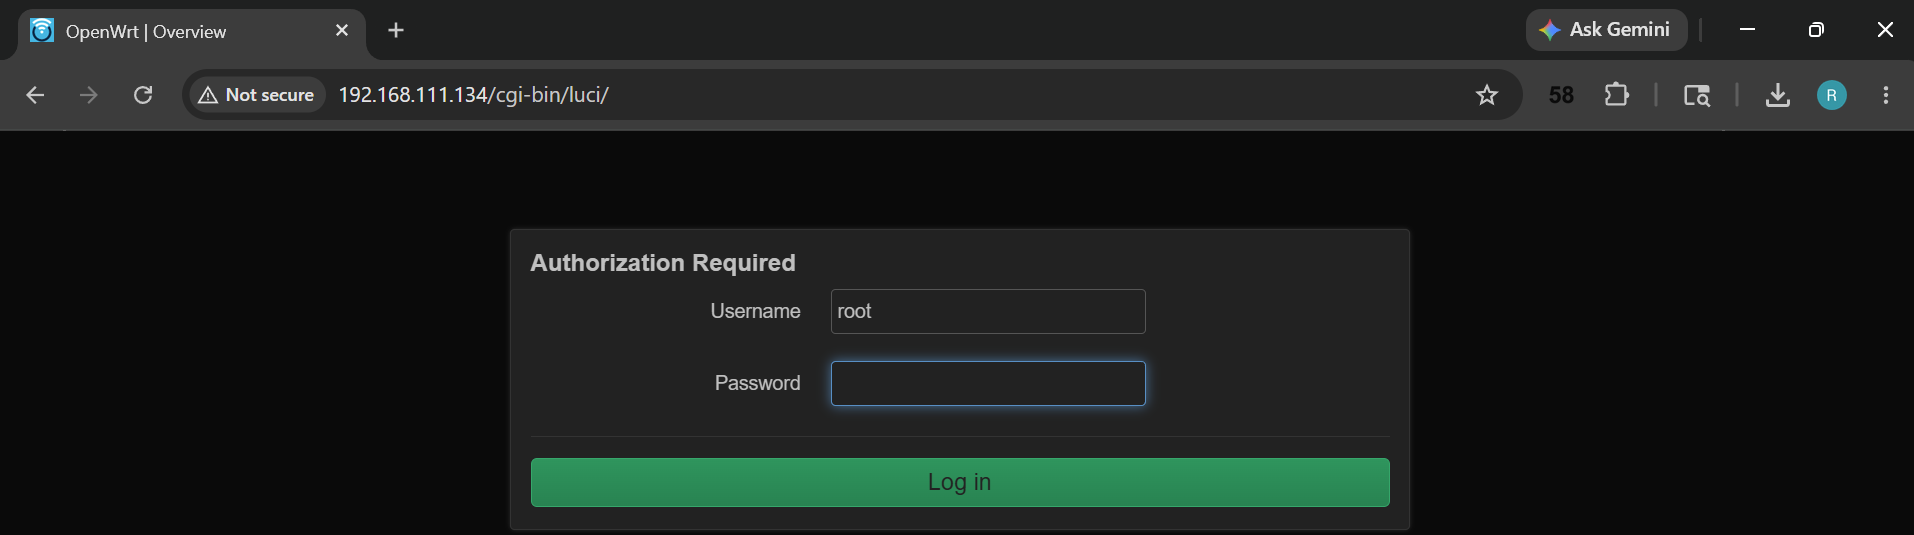
\includegraphics[width=0.45\textwidth]{figures/luci1.png}
\caption{Accessible LuCI web management login page}
\label{fig:luci1}
\end{figure}
\begin{figure}[H]
\centering
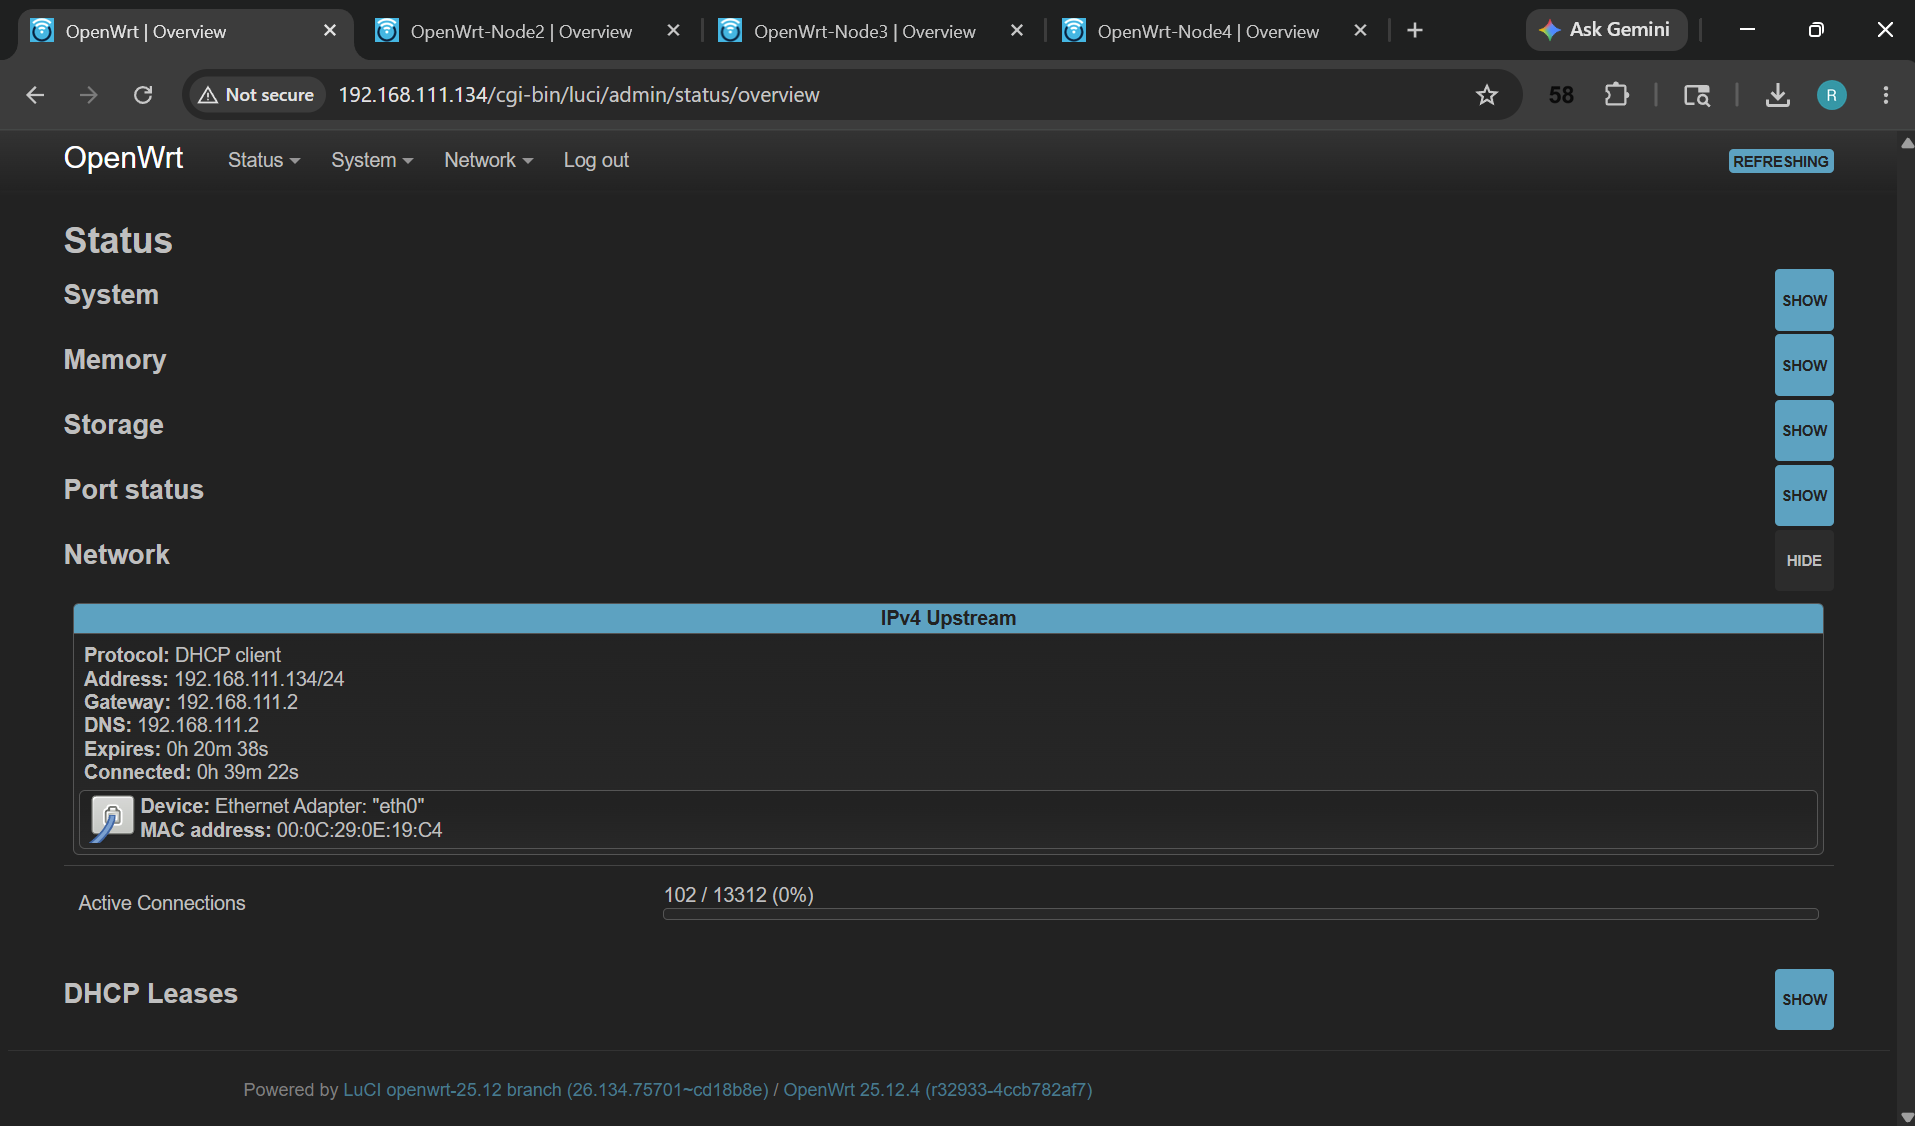
\includegraphics[width=0.45\textwidth]{figures/luci2.png}
\caption{Accessible LuCI web management interface through VMware NAT networking.}
\label{fig:luci2}
\end{figure}

\section{Multi-Node Mesh Backbone Construction}

\subsection{Dual-Interface Mesh Backbone}

After establishing a stable baseline, a second virtual adapter was reintroduced using VMware host-only networking.

The second interface was assigned as a dedicated mesh backbone network:

\begin{lstlisting}
uci set network.mesh=interface
uci set network.mesh.proto='static'
uci set network.mesh.device='eth1'
uci set network.mesh.ipaddr='10.10.10.1'
uci set network.mesh.netmask='255.255.255.0'
uci commit network
/etc/init.d/network restart
\end{lstlisting}

Resulting topology:

\begin{table}[H]
\centering
\caption{Dual-Interface OpenWrt Topology}
\begin{tabular}{|l|l|l|}
\hline
Interface & Address & Purpose \\ \hline
eth0 & 192.168.111.x & VMware NAT / WAN \\ \hline
eth1 & 10.10.10.x & Internal mesh backbone \\ \hline
\end{tabular}
\end{table}

Routing verification confirmed correct segmentation:

\begin{lstlisting}
default via 192.168.111.2 dev eth0
10.10.10.0/24 dev eth1
\end{lstlisting}

\begin{figure}[H]
\centering
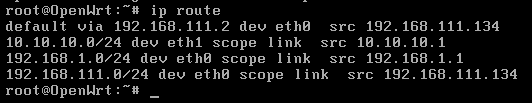
\includegraphics[width=0.45\textwidth]{figures/node1-route.png}
\caption{Validated OpenWrt Node 1 routing table showing WAN and mesh backbone separation.}
\label{fig:ip-route}
\end{figure}


\subsection{VM Cloning Strategy}

Instead of reinstalling OpenWrt repeatedly, a stable “golden image” virtual machine was cloned using VMware full-clone functionality.

Resulting nodes included:

\begin{itemize}
    \item OpenWrt-Node1
    \item OpenWrt-Node2
    \item OpenWrt-Node3
    \item OpenWrt-Node4
\end{itemize}

Each node received:

\begin{itemize}
    \item Unique hostname
    \item Unique mesh backbone address
    \item VMware-generated MAC address
\end{itemize}

\subsection{Four-Node Mesh Backbone Validation}

The resulting mesh backbone addressing scheme included:

\begin{table}[H]
\centering
\caption{Four-Node Mesh Backbone Addressing}
\begin{tabular}{|l|l|}
\hline
Node & Mesh Address \\ \hline
OpenWrt-Node1 & 10.10.10.1 \\ \hline
OpenWrt-Node2 & 10.10.10.2 \\ \hline
OpenWrt-Node3 & 10.10.10.3 \\ \hline
OpenWrt-Node4 & 10.10.10.4 \\ \hline
\end{tabular}
\end{table}

Connectivity testing was performed between all nodes using ICMP echo requests.

Successful bidirectional communication was verified between all nodes with:

\begin{itemize}
    \item Zero packet loss
    \item Stable latency
    \item Successful route propagation
\end{itemize}

The successful validation demonstrated:

\begin{itemize}
    \item Stable Layer 2 adjacency
    \item Functional Layer 3 routing
    \item Operational VMware host-only backbone networking
    \item Successful multi-node OpenWrt virtualization
\end{itemize}

\begin{figure}[H]
\centering
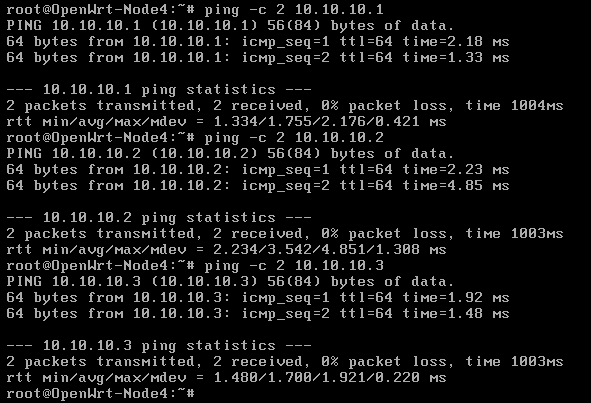
\includegraphics[width=0.45\textwidth]{figures/node4-ping.png}
\caption{Successful four-node mesh backbone connectivity validation.}
\label{fig:node4-ping}
\end{figure}

\subsection{Sequential Startup and DHCP Convergence}

Initial simultaneous startup of cloned nodes produced temporary WAN IP duplication behavior within the VMware NAT network.

Multiple nodes briefly inherited identical DHCP leases from previous cloned states.

This behavior was mitigated by sequential node startup. Sequential startup allowed VMware DHCP services to converge properly and assign unique WAN addresses based on MAC address differentiation.

Final WAN assignments stabilized as:

\begin{itemize}
    \item Node1: 192.168.111.134
    \item Node2: 192.168.111.136
    \item Node3: 192.168.111.137
    \item Node4: 192.168.111.138
\end{itemize}

This demonstrated:

\begin{itemize}
    \item DHCP lease convergence behavior
    \item Temporary ARP instability during cloned startup
    \item Virtualization timing dependencies
    \item Successful MAC-based lease differentiation
\end{itemize}

\subsection{IPv6 Duplicate Address Detection Behavior}

During sequential startup of cloned nodes, OpenWrt repeatedly reported IPv6 duplicate address detection warnings:

\begin{lstlisting}
IPv6 duplicate address detected
\end{lstlisting}

Despite repeated IPv6 duplicate detection events:

\begin{itemize}
    \item IPv4 routing remained stable
    \item Mesh backbone communication remained operational
    \item Node-to-node connectivity was unaffected
\end{itemize}

This behavior represents an important operational consideration for cloned embedded router deployments and virtualized distributed networking systems.

\begin{figure}[H]
\centering
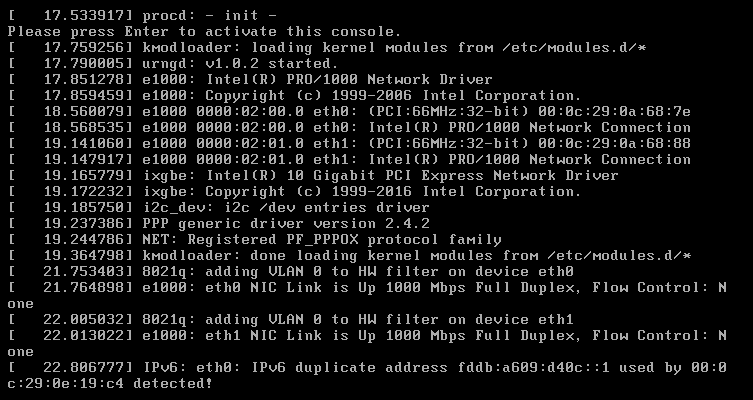
\includegraphics[width=0.45\textwidth]{figures/ipv6error.png}
\caption{Observed IPv6 duplicate address detection during sequential startup of cloned OpenWrt nodes.}
\label{fig:ipv6error}
\end{figure}

\section{BATMAN-adv Mesh Routing Deployment}

\subsection{BATMAN-adv Installation}

After the successful construction of the four-node OpenWrt backbone topology, the BATMAN-adv routing protocol was deployed to provide dynamic Layer 2 mesh routing functionality.

The following packages were installed on all nodes:

\begin{lstlisting}
apk add kmod-batman-adv batctl luci-proto-batman-adv
\end{lstlisting}

Successful installation loaded the BATMAN kernel module dynamically:

\begin{lstlisting}
lsmod | grep batman
\end{lstlisting}

The BATMAN mesh interface was manually initialized:

\begin{lstlisting}
modprobe batman-adv
ip link add name bat0 type batadv
ip link set up dev bat0
\end{lstlisting}

The dedicated mesh transport interface was attached to BATMAN:

\begin{lstlisting}
batctl meshif bat0 if add eth1
\end{lstlisting}

\begin{figure}[H]
\centering
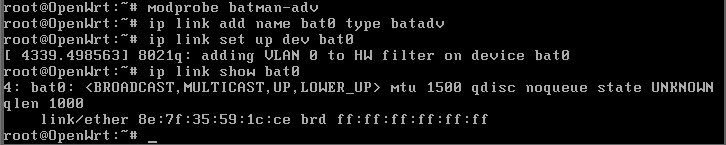
\includegraphics[width=0.48\textwidth]{figures/bat0add.png}
\caption{Successful initialization of the BATMAN-adv virtual mesh interface.}
\label{fig:bat0add}
\end{figure}

\subsection{Dynamic Neighbor Discovery}

BATMAN dynamically discovered neighboring routers using:

\begin{lstlisting}
batctl meshif bat0 n
\end{lstlisting}

Originator propagation tables were observed using:

\begin{lstlisting}
batctl meshif bat0 o
\end{lstlisting}

\begin{figure}[H]
\centering
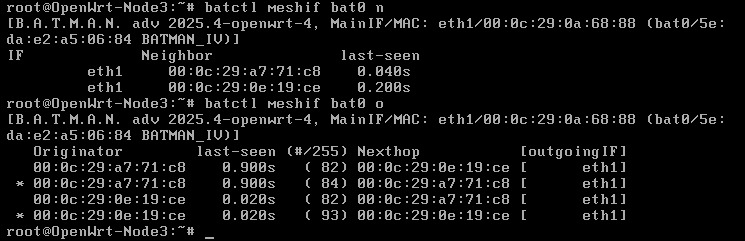
\includegraphics[width=0.48\textwidth]{figures/mesh-routes.png}
\caption{BATMAN-adv originator routing tables dynamically populated across the mesh.}
\label{fig:meshroutes}
\end{figure}

\subsection{Four-Node Mesh Convergence}

All four OpenWrt nodes successfully joined the distributed BATMAN mesh.

The resulting deployment demonstrated:

\begin{itemize}
    \item Autonomous neighbor discovery
    \item Dynamic route propagation
    \item Persistent distributed convergence
    \item Self-healing mesh behavior
\end{itemize}

\begin{figure}[H]
\centering
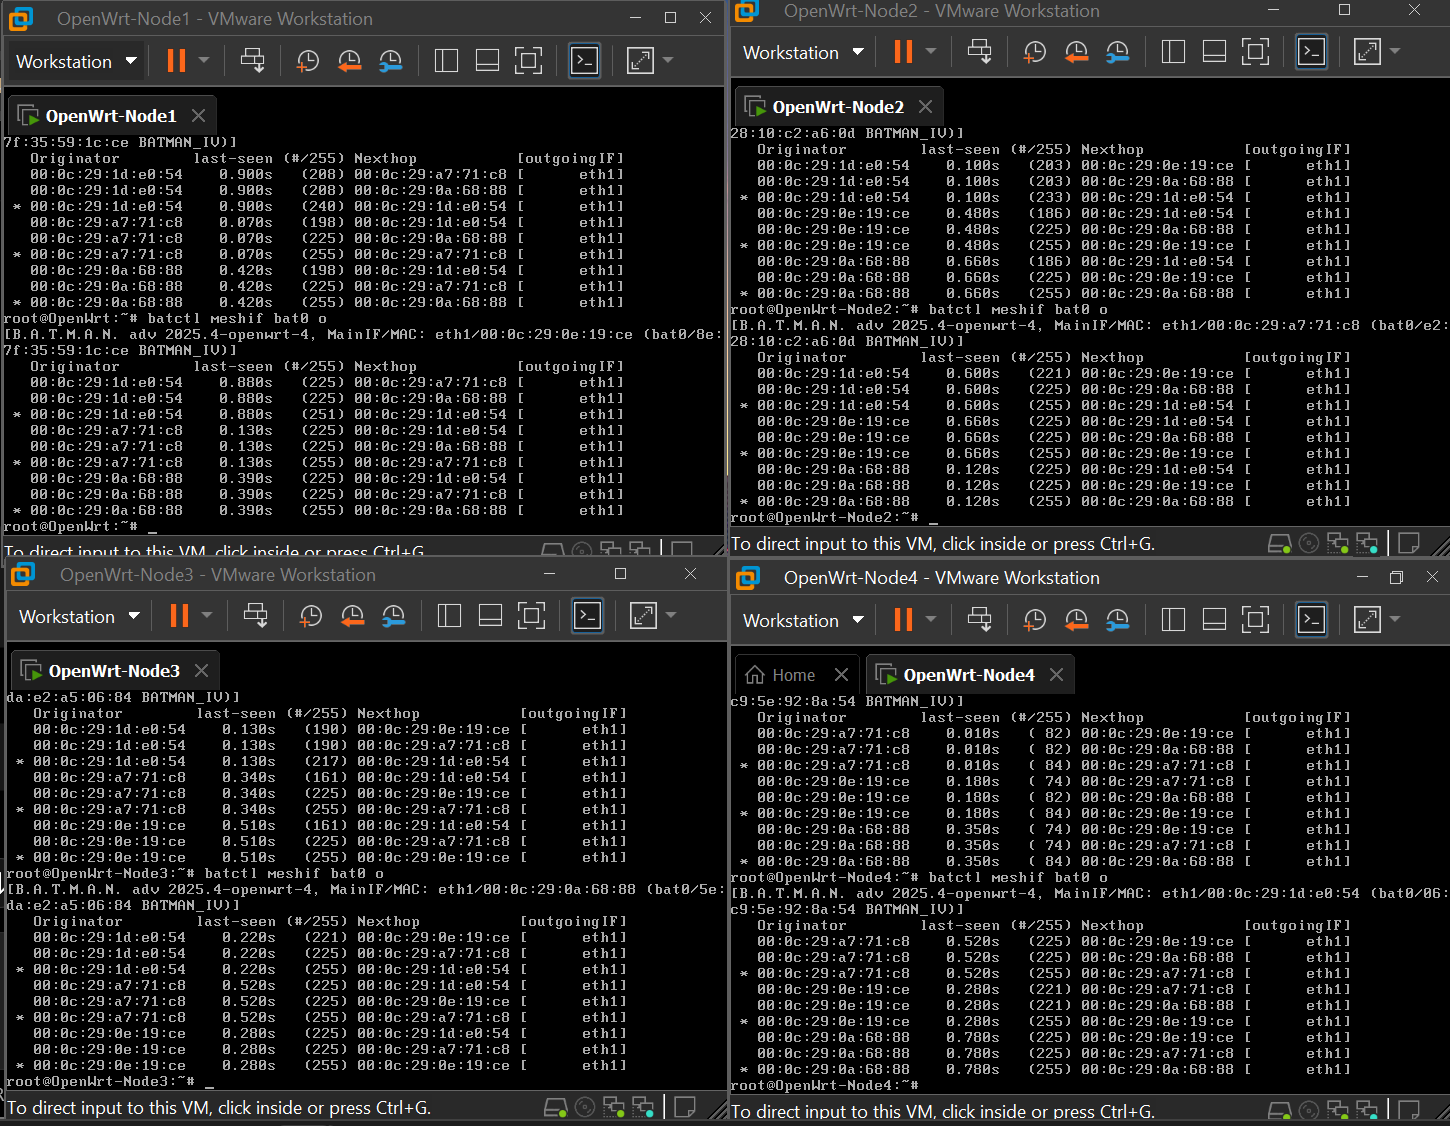
\includegraphics[width=0.49\textwidth]{figures/pre-fail-top.png}
\caption{Stable four-node BATMAN-adv mesh topology before failure testing.}
\label{fig:prefail}
\end{figure}

\subsection{Node Failure and Reconvergence}

One node was intentionally powered off during operation to evaluate mesh resilience behavior.

Immediately after failure:

\begin{itemize}
    \item Neighbor tables updated dynamically
    \item Stale originators were removed
    \item Remaining nodes maintained connectivity
\end{itemize}

\begin{figure}[H]
\centering
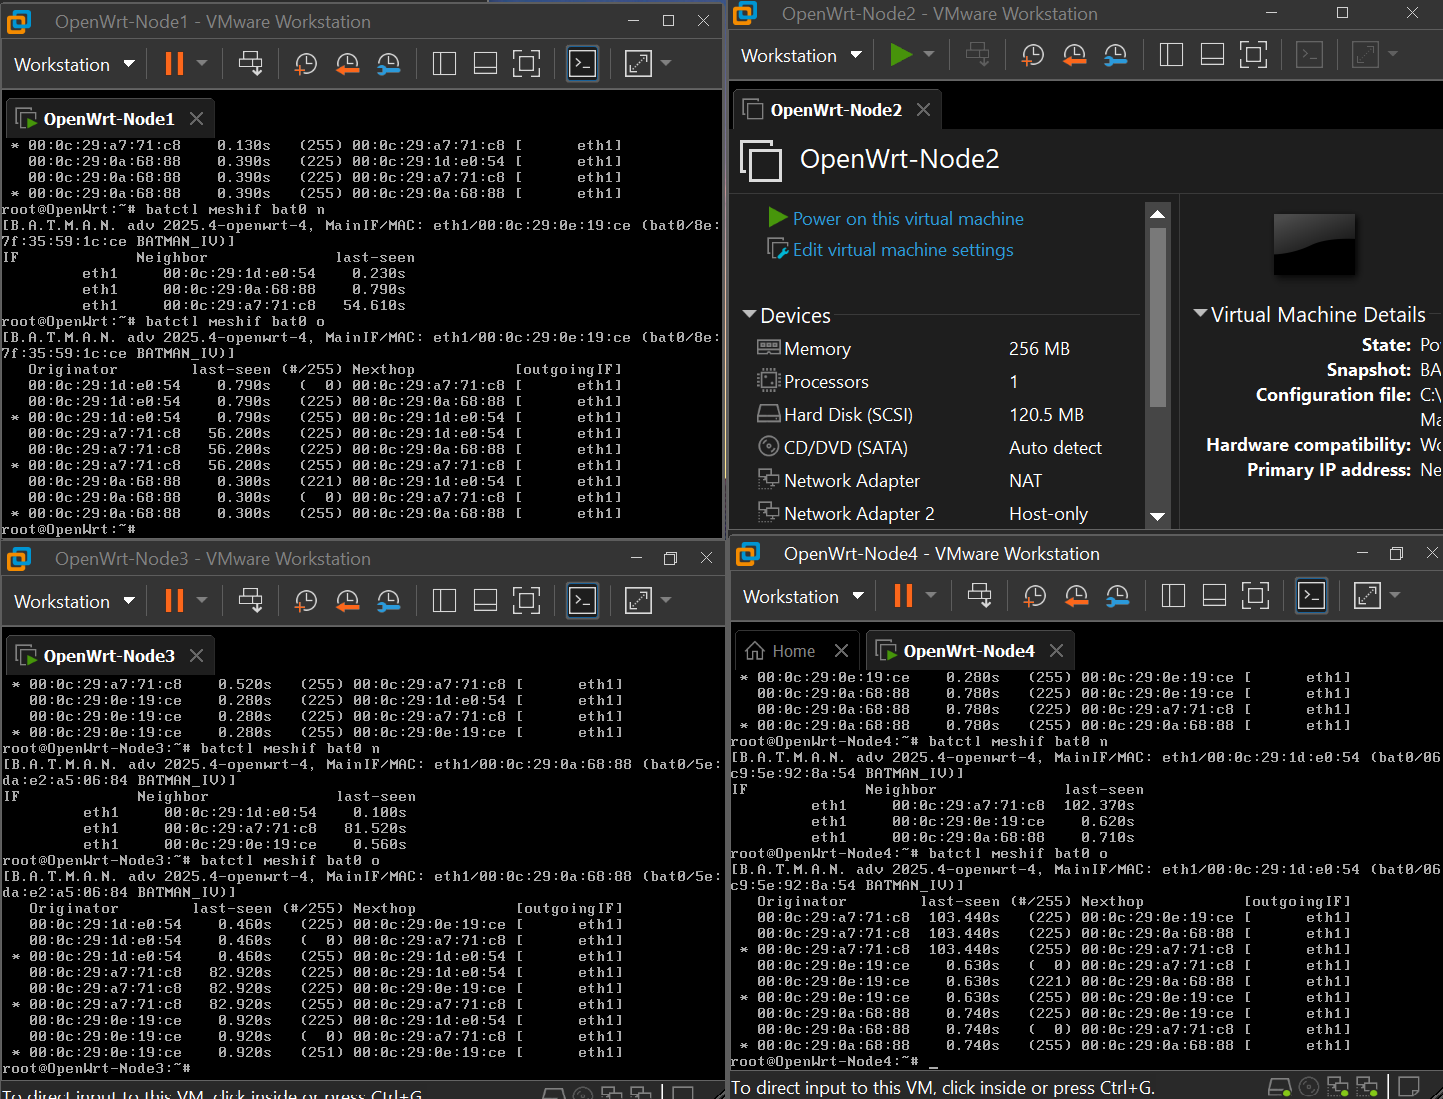
\includegraphics[width=0.49\textwidth]{figures/post-fail-top.png}
\caption{BATMAN topology immediately following intentional node failure.}
\label{fig:postfail}
\end{figure}

\subsection{Node Reintegration}

After reboot, the failed node automatically rejoined the distributed mesh without manual reconfiguration.

\begin{figure}[H]
\centering
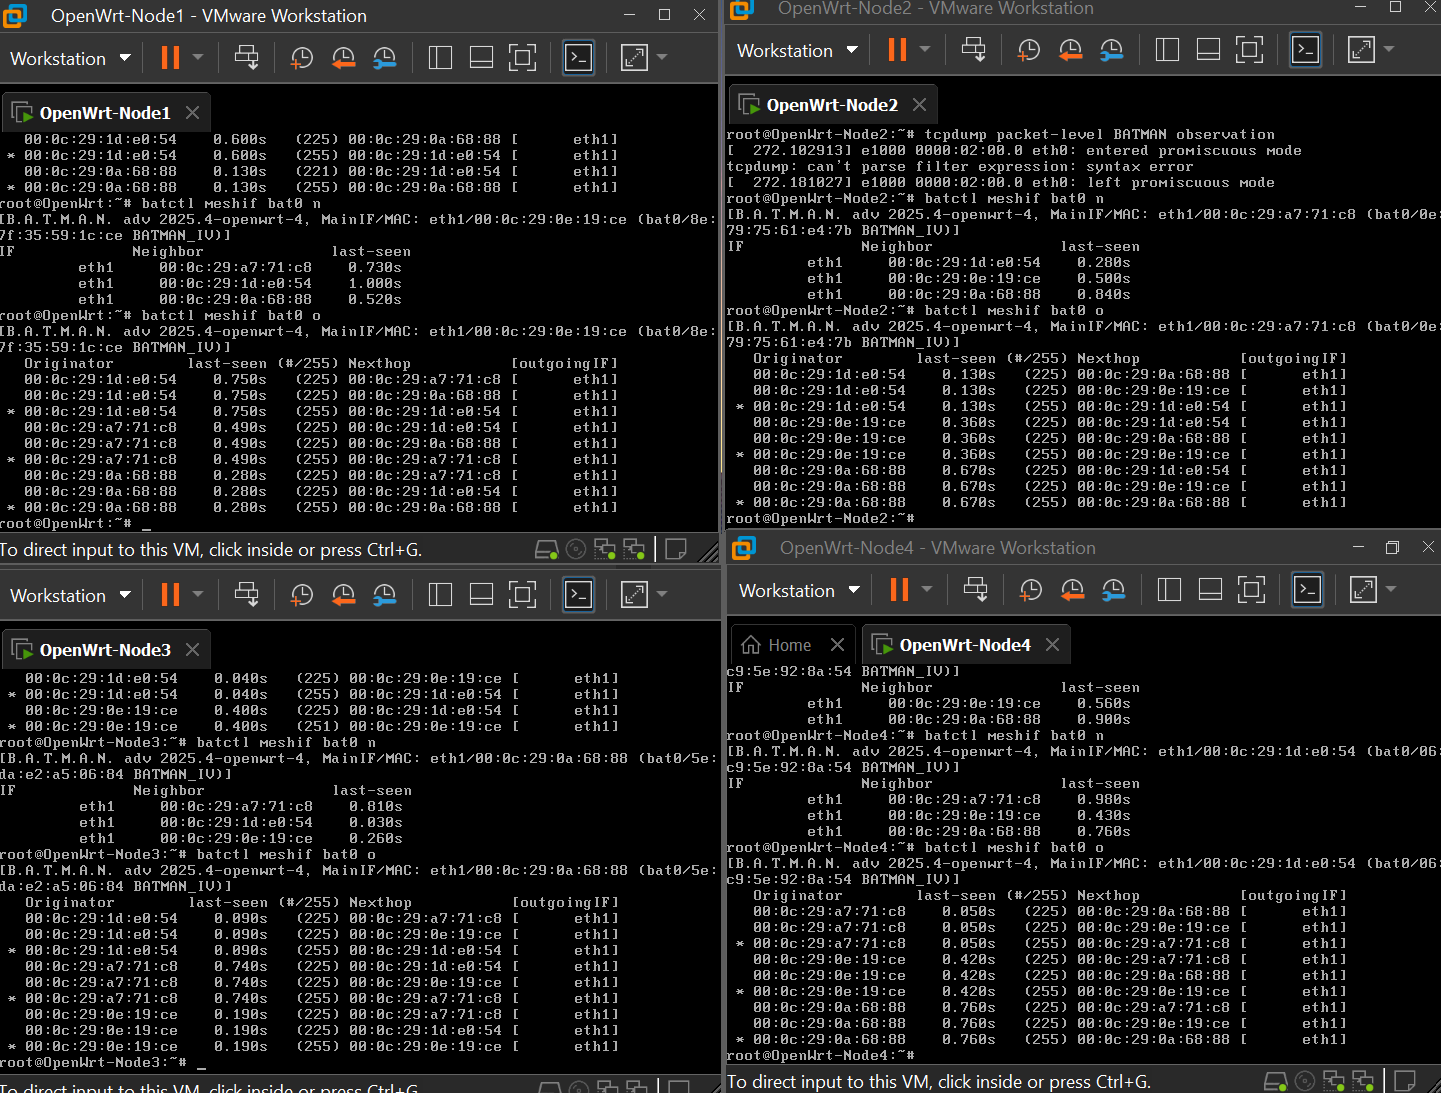
\includegraphics[width=0.49\textwidth]{figures/post-fail-top-post-boot.png}
\caption{Automatic BATMAN mesh reconvergence after node restoration.}
\label{fig:postboot}
\end{figure}

\subsection{Persistent BATMAN Configuration}

Persistent deployment was implemented using OpenWrt UCI configuration:

\begin{lstlisting}
uci set network.bat0=interface
uci set network.bat0.proto='batadv'
uci set network.bat0.routing_algo='BATMAN_IV'

uci set network.mesh_bat=interface
uci set network.mesh_bat.proto='batadv_hardif'
uci set network.mesh_bat.master='bat0'
uci set network.mesh_bat.device='eth1'

uci commit network
\end{lstlisting}

After reboot, all nodes automatically:
\begin{itemize}
    \item Recreated bat0
    \item Reattached eth1
    \item Rediscovered neighbors
    \item Rejoined the mesh
\end{itemize}

\subsection{BATMAN Native Ping and Traceroute}

BATMAN-native connectivity was validated using:

\begin{lstlisting}
batctl meshif bat0 ping <neighbor MAC>
\end{lstlisting}

Traceroute functionality was validated using:

\begin{lstlisting}
batctl meshif bat0 traceroute <neighbor MAC>
\end{lstlisting}

\begin{figure}[H]
\centering
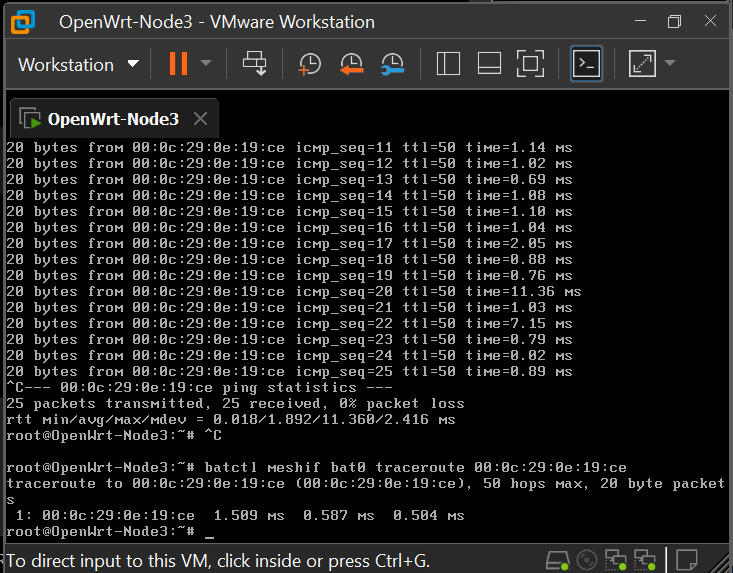
\includegraphics[width=0.48\textwidth]{figures/traceroute.png}
\caption{BATMAN-native traceroute across the distributed mesh topology.}
\label{fig:traceroute}
\end{figure}

\subsection{MTU Optimization and Fragmentation Analysis}

BATMAN generated warnings indicating insufficient MTU allocation on the transport interface.

Initial configuration:

\begin{itemize}
    \item eth1 MTU: 1500
    \item bat0 MTU: 1500
\end{itemize}

The transport interface MTU was increased experimentally:

\begin{lstlisting}
ip link set dev eth1 mtu 1532
\end{lstlisting}

Following optimization:
\begin{itemize}
    \item Neighbor discovery remained stable
    \item BATMAN forwarding persisted
    \item Packet loss remained zero
\end{itemize}

Interestingly, bat0 continued operating at MTU 1500 while eth1 operated at MTU 1532.

\begin{figure}[H]
\centering
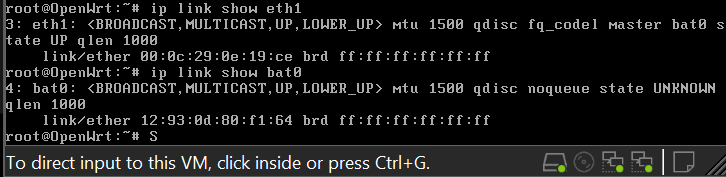
\includegraphics[width=0.48\textwidth]{figures/old-mtu.png}
\caption{Initial BATMAN deployment with insufficient MTU allocation.}
\label{fig:oldmtu}
\end{figure}

\begin{figure}[H]
\centering
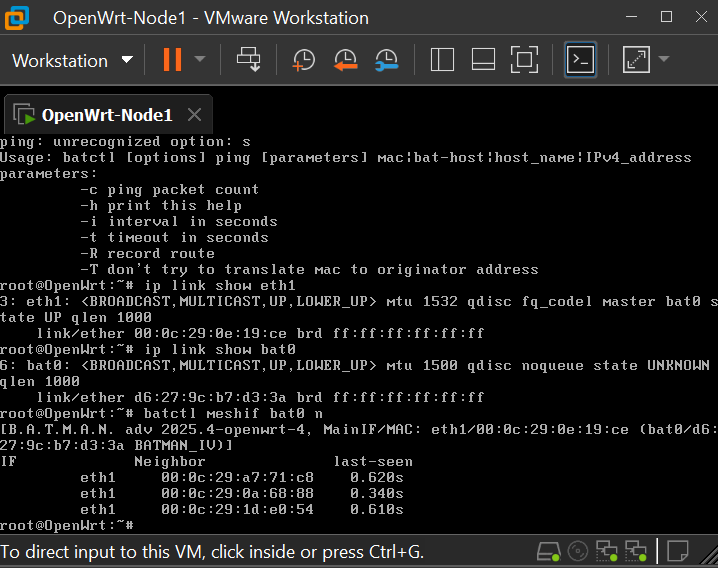
\includegraphics[width=0.48\textwidth]{figures/new-mtu.png}
\caption{Stable BATMAN operation following MTU optimization.}
\label{fig:newmtu}
\end{figure}

\subsection{Management-Plane Addressing Issues}

During virtual-machine cloning, multiple nodes temporarily inherited overlapping management-plane identities.

Observed effects included:
\begin{itemize}
    \item Duplicate DHCP assignments
    \item Ambiguous LuCI access
    \item IPv6 duplicate-address warnings
\end{itemize}

Despite management-plane ambiguity, the BATMAN forwarding plane remained fully operational.

\begin{figure}[H]
\centering
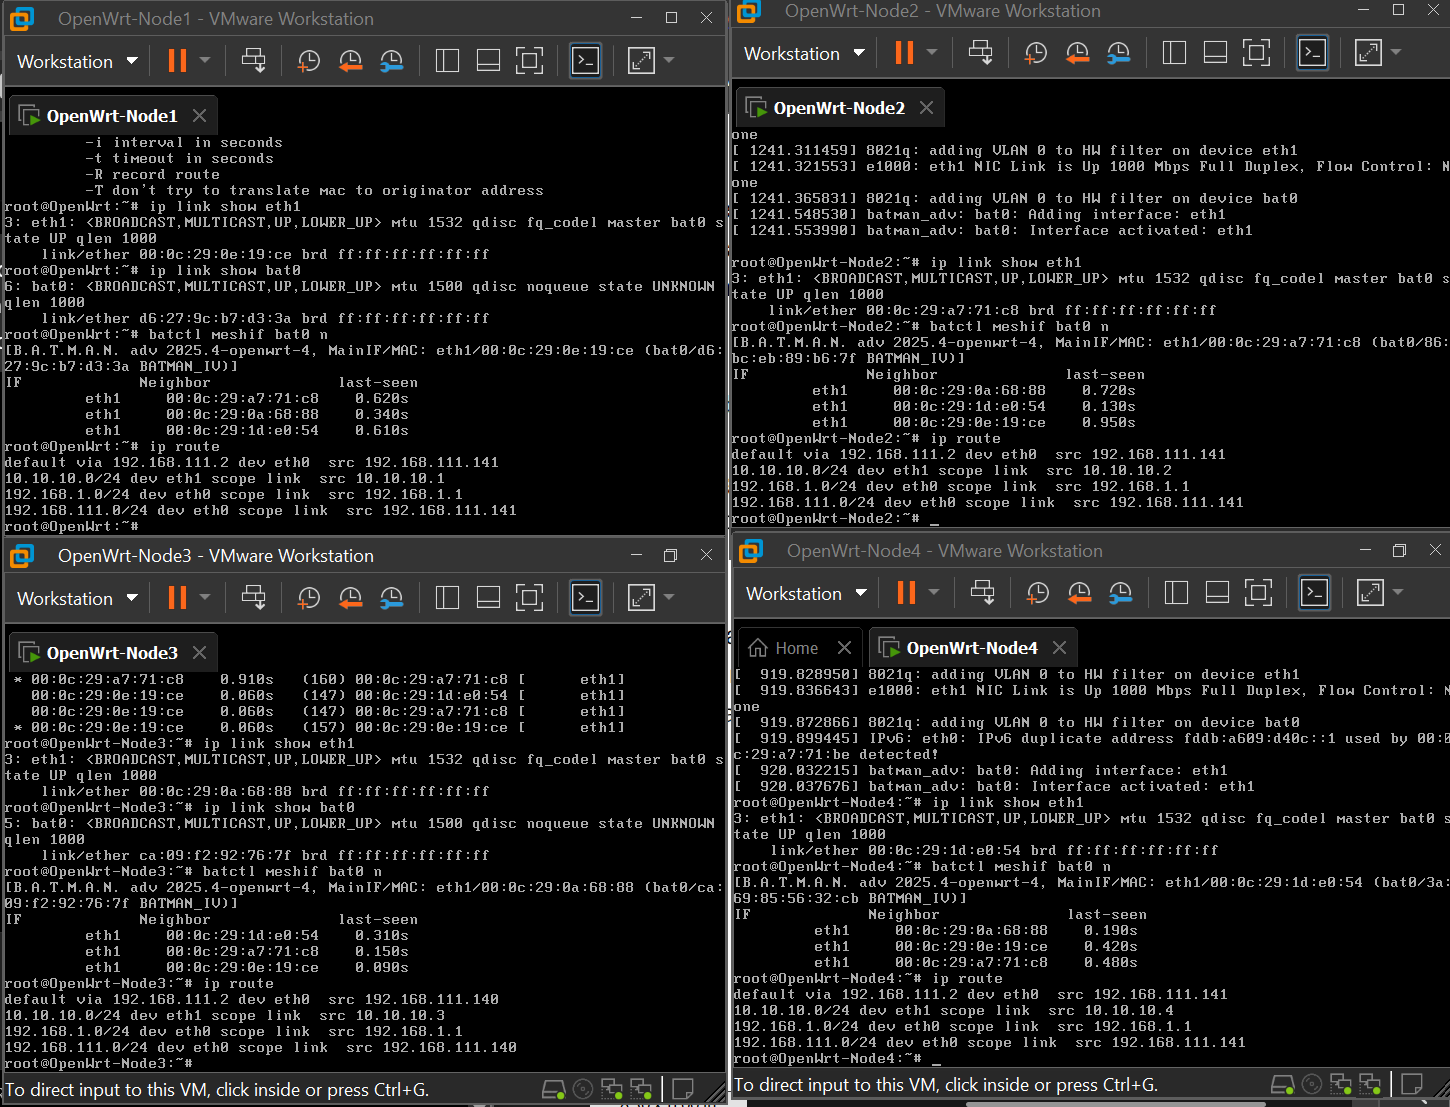
\includegraphics[width=0.48\textwidth]{figures/nodeip-issue.png}
\caption{Management-plane addressing conflicts during cloned OpenWrt deployment.}
\label{fig:nodeipissue}
\end{figure}

\section{LibreMesh Firmware and Wireless Hardware Requirements}

The LibreMesh project provides prebuilt OpenWrt-based firmware images designed specifically for decentralized wireless mesh deployments.

Installation procedures and firmware selection guidance were obtained from the official LibreMesh documentation and firmware selector platform.

LibreMesh installation generally requires:

\begin{itemize}
    \item OpenWrt-supported hardware
    \item At least 16 MB flash storage
    \item At least 128 MB RAM
    \item One operational 2.4 GHz wireless radio
    \item One operational 5 GHz wireless radio
\end{itemize}

The dual-radio recommendation exists because LibreMesh commonly separates:

\begin{itemize}
    \item Client-access traffic
    \item Mesh-backhaul traffic
\end{itemize}

Typical deployments utilize:

\begin{itemize}
    \item 2.4 GHz radios for local client access and extended range
    \item 5 GHz radios for higher-throughput mesh backhaul links
\end{itemize}

LibreMesh firmware may be obtained using:

\begin{itemize}
    \item LibreMesh Firmware Selector
    \item Precompiled firmware archives
    \item Custom OpenWrt ImageBuilder compilation
\end{itemize}

The project initially investigated whether full LibreMesh wireless meshing could be reproduced entirely inside VMware virtualization.

However, VMware virtual network adapters emulate Ethernet devices rather than physical IEEE 802.11 wireless radios.

As a result, VMware virtual adapters do not provide:

\begin{itemize}
    \item True wireless PHY behavior
    \item RF channel negotiation
    \item Wireless beaconing
    \item 802.11s mesh operation
    \item Ad-hoc wireless functionality
    \item Monitor-mode radio capabilities
\end{itemize}

Although BATMAN-adv operated successfully over virtual Ethernet interfaces, this represented a Layer 2 routed mesh simulation rather than a true wireless LibreMesh deployment.

The virtualized environment therefore successfully validated:

\begin{itemize}
    \item Distributed BATMAN routing behavior
    \item Dynamic neighbor discovery
    \item Autonomous route propagation
    \item Persistent distributed convergence
\end{itemize}

However, full LibreMesh wireless operation will require physical wireless hardware during the Raspberry Pi deployment phase.

\section{Configuration Export and Deployment Reproducibility}

To satisfy reproducibility requirements, configuration artifacts and operational mesh-state information were exported directly from all OpenWrt nodes.

The exported artifacts included:

\begin{itemize}
    \item Persistent OpenWrt UCI configuration files
    \item BATMAN neighbor tables
    \item BATMAN originator tables
    \item Routing tables
    \item Interface-state information
    \item Installed package inventories
\end{itemize}

A reusable export automation script was developed to simplify artifact extraction across all nodes.

The script automatically:
\begin{itemize}
    \item Collected configuration files
    \item Captured BATMAN operational state
    \item Archived deployment artifacts
    \item Generated compressed export bundles
\end{itemize}

The resulting deployment archives were extracted remotely from the OpenWrt nodes using SSH and SCP.

\subsection{Automated Configuration Export Script}

The following script was deployed on all OpenWrt nodes:

\begin{lstlisting}
#!/bin/sh

NODE_NAME="$(cat /proc/sys/kernel/hostname)"
OUTDIR="/root/config-export"
ARCHIVE="/root/${NODE_NAME}-config-export.tar.gz"

mkdir -p "$OUTDIR"

cp /etc/config/network \
"$OUTDIR/network-${NODE_NAME}"

cp /etc/config/system \
"$OUTDIR/system-${NODE_NAME}"

cp /etc/config/firewall \
"$OUTDIR/firewall-${NODE_NAME}"

cp /etc/config/dhcp \
"$OUTDIR/dhcp-${NODE_NAME}"

batctl meshif bat0 if > \
"$OUTDIR/batman-if-${NODE_NAME}.txt"

batctl meshif bat0 n > \
"$OUTDIR/batman-neighbors-${NODE_NAME}.txt"

batctl meshif bat0 o > \
"$OUTDIR/batman-originators-${NODE_NAME}.txt"

ip addr > \
"$OUTDIR/ip-addr-${NODE_NAME}.txt"

ip route > \
"$OUTDIR/ip-route-${NODE_NAME}.txt"

apk list --installed > \
"$OUTDIR/packages-${NODE_NAME}.txt"

tar -czf "$ARCHIVE" \
-C /root config-export
\end{lstlisting}

\subsection{Windows and Linux Script Compatibility Issues}

During deployment automation, shell scripts transferred from Windows systems to OpenWrt routers initially failed with:

\begin{lstlisting}
-ash: /root/export-config.sh: not found
\end{lstlisting}

Investigation revealed that the script contained Windows CRLF line endings rather than Linux LF line endings.

This caused BusyBox ash to misinterpret the script interpreter line:

\begin{lstlisting}
#!/bin/sh^M
\end{lstlisting}

The issue was corrected using:

\begin{lstlisting}
sed -i 's/\r$//' /root/export-config.sh
\end{lstlisting}

This represented an important interoperability consideration between Windows administrative systems and embedded Linux networking environments.

\subsection{SSH and SCP Artifact Extraction}

Configuration archives were remotely extracted from OpenWrt nodes using SCP over SSH.

Modern Windows SCP implementations attempted to default to SFTP mode, which was unsupported by the lightweight OpenWrt Dropbear deployment.

Observed error:

\begin{lstlisting}
subsystem request failed on channel 0
scp: Connection closed
\end{lstlisting}

Successful extraction required forcing legacy SCP protocol mode:

\begin{lstlisting}
scp -O root@192.168.111.x:/root/archive.tar.gz .
\end{lstlisting}

This demonstrated another operational limitation common within lightweight embedded Linux distributions where full SFTP subsystems are often omitted to conserve storage space and memory resources.

\section{Git-Based Collaborative Configuration Management}

To improve reproducibility, collaboration, and long-term configuration management, the project artifacts were integrated into a Git-based version-control workflow using GitHub.

The repository centralized:

\begin{itemize}
    \item LaTeX report source files
    \item Figures and screenshots
    \item OpenWrt configuration exports
    \item BATMAN operational logs
    \item Deployment scripts
    \item Supporting documentation
\end{itemize}

This approach allowed multiple project participants to:

\begin{itemize}
    \item Retrieve synchronized project files
    \item Contribute modifications collaboratively
    \item Maintain deployment history
    \item Track configuration revisions
    \item Restore previous project states if necessary
\end{itemize}

\subsection{Repository Initialization}

A new local Git repository was initialized within the project directory:

\begin{lstlisting}
git init
\end{lstlisting}

A \texttt{.gitignore} file was created to exclude temporary LaTeX compilation artifacts including:

\begin{lstlisting}
*.aux
*.log
*.out
*.toc
*.synctex.gz
\end{lstlisting}

Project files were staged and committed locally:

\begin{lstlisting}
git add .
git commit -m "Initial LibreMesh project upload"
\end{lstlisting}

The local repository was then connected to a remote GitHub repository:

\begin{lstlisting}
git remote add origin \
https://github.com/<user>/<repo>.git
\end{lstlisting}

The repository was uploaded using:

\begin{lstlisting}
git branch -M main
git push -u origin main
\end{lstlisting}

\subsection{Repository Structure}

The resulting repository structure organized project artifacts into separate directories:

\begin{lstlisting}
EC3730-Pro/
|-archive/
|-report/
|-virtual machines/
|-EC3730_Final_Project.pdf
|-README.md
\end{lstlisting}

This structure separated:
\begin{itemize}
    \item Documentation
    \item Deployment scripts
    \item Configuration archives
    \item Experimental artifacts
\end{itemize}

\subsection{Collaborative Workflow}

Additional project participants could retrieve the repository using:

\begin{lstlisting}
git clone \
https://github.com/<user>/<repo>.git
\end{lstlisting}

Once cloned locally, collaborators could synchronize project updates using:

\begin{lstlisting}
git pull
\end{lstlisting}

Modified files could then be uploaded back to the shared repository using:

\begin{lstlisting}
git add .
git commit -m "Describe changes"
git push
\end{lstlisting}

This created a distributed collaborative workflow allowing all participants to maintain synchronized copies of the deployment environment and report documentation.

\subsection{Version-Control Benefits}

Git-based version control provided several operational advantages during experimentation:

\begin{itemize}
    \item Distributed backup of project artifacts
    \item Historical tracking of configuration changes
    \item Simplified collaboration between participants
    \item Recovery from accidental file modification
    \item Improved reproducibility of deployment procedures
\end{itemize}

The integration of Git-based workflow management significantly improved the maintainability and reproducibility of the overall mesh-network deployment project.

\section{Raspberry Pi Deployment}

\subsection{Custom LibreMesh Firmware Image Generation}

To simplify deployment onto Raspberry Pi 5 hardware, a custom LibreMesh firmware image was generated using the LibreMesh firmware builder.

The firmware image targeted the Raspberry Pi 5 platform:

\begin{itemize}
    \item Platform: bcm27xx/bcm2712
    \item Device: Raspberry Pi 5
    \item OpenWrt Version: 25.12.4
    \item LibreMesh Feed Branch: master
    \item Routing Protocol: BATMAN-adv
\end{itemize}

Additional management and diagnostic packages were included during image generation:

\begin{itemize}
    \item BATMAN-adv kernel modules
    \item LuCI web administration interface
    \item SSH services
    \item TCPDump
    \item iPerf3
    \item Curl
    \item Wget
    \item Nano
    \item Htop
    \item JSON query utilities
\end{itemize}

The LibreMesh image builder also supports execution of a first-boot script through the OpenWrt \texttt{uci-defaults} mechanism. This allows nodes to self-configure immediately after their initial boot sequence.

\subsection{Automated First-Boot Provisioning}

A custom first-boot script named:

\begin{verbatim}
EC3730_firstboot_router_ap
\end{verbatim}

was developed to automatically provision a Raspberry Pi LibreMesh node.

The script performs the following actions:

\begin{itemize}
    \item Sets a predefined hostname
    \item Creates centralized log directories
    \item Verifies installed package availability
    \item Configures a common EC3730 wireless network
    \item Enables WPA2 wireless security
    \item Removes stale client-mode wireless configurations
    \item Preserves LibreMesh BATMAN-adv operation
    \item Adjusts DHCP address allocation behavior
    \item Creates mesh troubleshooting utilities
    \item Creates packet-capture utilities
    \item Creates automated connectivity testing utilities
    \item Generates deployment logs
\end{itemize}

The deployment standardizes all classroom nodes using:

\begin{center}
SSID: EC3730

Password: EC3730Mesh!
\end{center}

To improve address-management consistency, the DHCP pool is configured to begin allocating client leases at host offset 11. This reserves the first ten low host addresses for future infrastructure assignments and static device allocation.

The provisioning process also generates several operational support tools:

\begin{itemize}
    \item \texttt{check\_mesh.sh}
    \item \texttt{capture\_mesh.sh}
    \item \texttt{test\_connectivity.sh}
\end{itemize}

These scripts automate routine troubleshooting tasks including:

\begin{itemize}
    \item BATMAN neighbor verification
    \item BATMAN originator analysis
    \item Wireless status verification
    \item Routing-table inspection
    \item Packet capture generation
    \item Connectivity testing
\end{itemize}

Following firmware flashing and initial boot, a Raspberry Pi node can automatically transition into a managed LibreMesh deployment without requiring extensive manual configuration.

This approach significantly reduces deployment time, improves reproducibility, and minimizes configuration drift between participating mesh-network nodes.

\subsection{Firmware Flashing and Initial Boot}

After generating the customized LibreMesh firmware image, the image was written to a microSD card using the Rufus imaging utility.

Rufus is a Windows-based USB and disk imaging tool capable of writing raw operating-system images directly to removable storage devices. The utility was selected because of its simplicity, reliability, and compatibility with OpenWrt firmware images.

The deployment procedure consisted of the following steps:

\begin{enumerate}
    \item Download the customized LibreMesh/OpenWrt firmware image.
    \item Insert a microSD card into the deployment workstation.
    \item Launch Rufus.
    \item Select the target microSD card.
    \item Select the LibreMesh firmware image.
    \item Write the image to the microSD card.
    \item Insert the microSD card into the Raspberry Pi 5.
    \item Apply power and allow the initial boot process to complete.
\end{enumerate}

Following successful boot, the Raspberry Pi automatically initialized the LibreMesh software stack and wireless services.

Verification of successful deployment was performed by observing the appearance of the configured wireless network SSID. The node began broadcasting the deployment SSID:

\begin{center}
EC3730
\end{center}

Detection of the wireless network confirmed:

\begin{itemize}
    \item Successful firmware flashing
    \item Successful Raspberry Pi boot sequence
    \item Proper wireless-radio initialization
    \item Execution of LibreMesh configuration services
    \item Activation of the wireless access-point interface
\end{itemize}

Once the wireless network became visible, management access could be established through either:

\begin{itemize}
    \item Direct Ethernet connection
    \item Secure Shell (SSH)
    \item LuCI web interface
\end{itemize}

The appearance of the wireless SSID provided a simple operational validation that the device had transitioned from a freshly flashed system into an operational LibreMesh node.

\begin{figure}[htbp]
\centerline{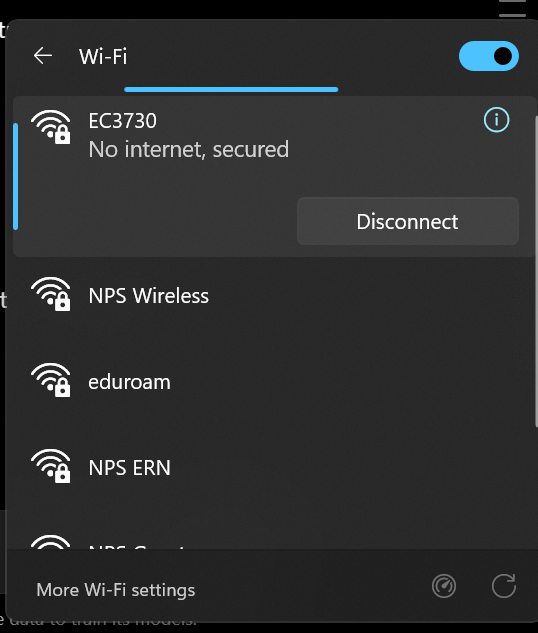
\includegraphics[width=\linewidth]{figures/raspberry-wifi.png}}
\caption{Raspberry Pi 5 broadcasting the EC3730 LibreMesh wireless network following initial boot.}
\label{fig:pi_ssid}
\end{figure}

\subsection{Exploring the Firmware}

Following successful deployment of the customized LibreMesh firmware image onto the Raspberry Pi 5, several verification and discovery procedures were performed to better understand the default LibreMesh configuration and confirm proper system operation.

The purpose of this exploration phase was to:

\begin{itemize}
    \item Verify successful firmware installation
    \item Confirm LibreMesh services were operational
    \item Identify automatically generated network interfaces
    \item Examine addressing behavior
    \item Validate wireless-radio functionality
    \item Investigate BATMAN-adv integration
    \item Establish a baseline configuration before further modifications
\end{itemize}

\subsubsection{Routing Table Inspection}

The first step was examination of the routing table using:

\begin{verbatim}
ip route
\end{verbatim}

The routing table revealed that LibreMesh automatically configured the node within the 10.13.0.0/16 network space and created an AnyGW interface for future gateway discovery and Internet-sharing functionality.

\begin{figure}[htbp]
\centerline{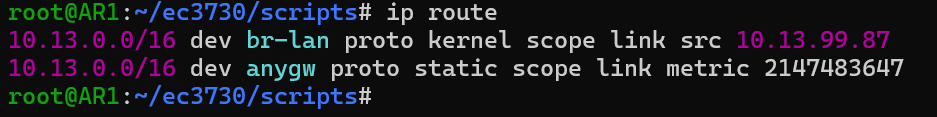
\includegraphics[width=\linewidth]{figures/ip-route-pi.png}}
\caption{LibreMesh routing table after initial boot.}
\label{fig:pi_route_table}
\end{figure}

Unlike the VMware BATMAN deployment, where addressing and routing were configured manually, LibreMesh automatically generated the routing configuration during the first boot sequence.

\subsubsection{Network Interface Analysis}

Network interfaces were examined using:

\begin{verbatim}
ip addr
\end{verbatim}

This inspection identified several automatically generated interfaces including:

\begin{itemize}
    \item br-lan
    \item anygw
    \item bat0
    \item wlan0-ap
\end{itemize}

The appearance of the \texttt{bat0} interface confirmed that BATMAN-adv had been initialized automatically by LibreMesh.

\begin{figure}[htbp]
\centerline{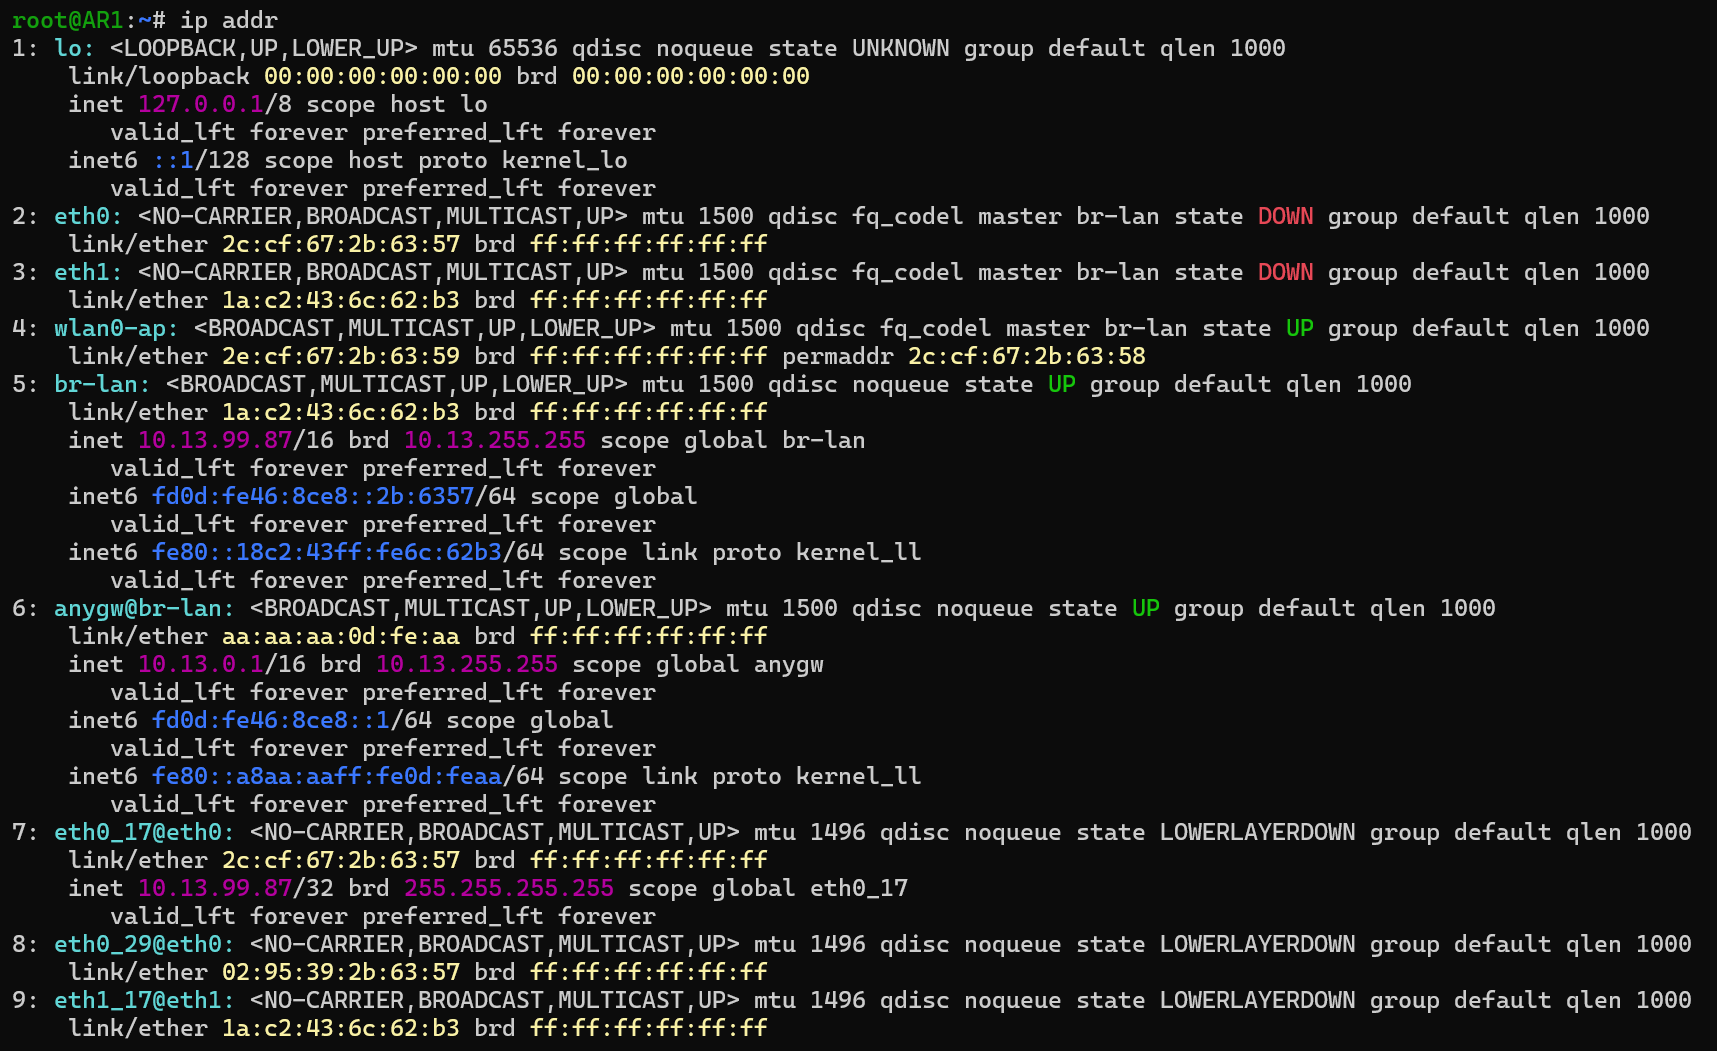
\includegraphics[width=\linewidth]{figures/ipaddr-q.png}}
\caption{Network interfaces generated automatically by LibreMesh.}
\label{fig:pi_ipaddr}
\end{figure}
\begin{figure}[htbp]
\centerline{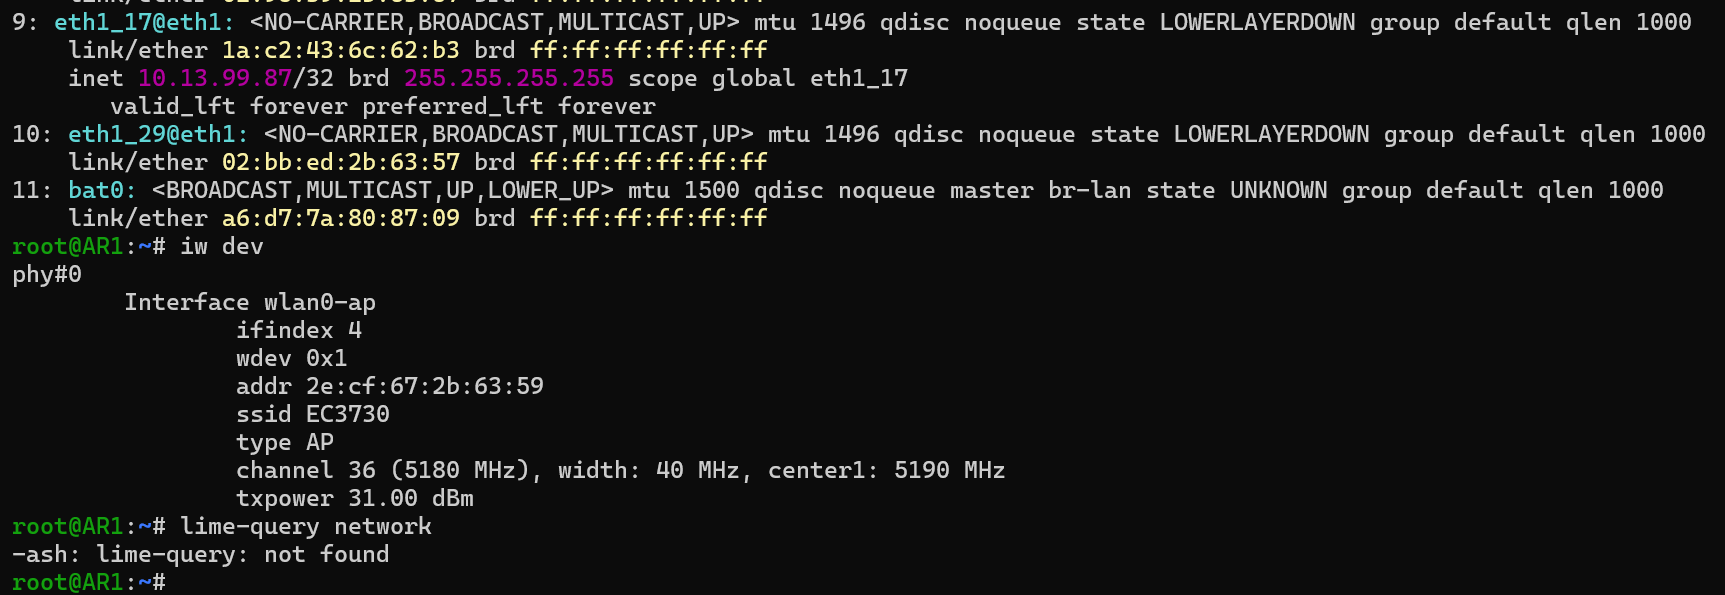
\includegraphics[width=\linewidth]{figures/ipaddr-qw.png}}
\caption{Network interfaces generated automatically by LibreMesh.}
\label{fig:pi_ipaddr}
\end{figure}

The node received the IPv4 address:

\begin{verbatim}
10.13.99.87/16
\end{verbatim}

which differs significantly from the manually assigned addresses used during the virtualized OpenWrt mesh-network deployment.

\subsubsection{Wireless Interface Verification}

Wireless functionality was verified using:

\begin{verbatim}
iw dev
\end{verbatim}

Results showed that LibreMesh successfully configured the Raspberry Pi wireless subsystem and created an access-point interface.

The configured deployment SSID:

\begin{verbatim}
EC3730
\end{verbatim}

was actively broadcast on channel 36 within the 5 GHz frequency band.

\begin{figure}[htbp]
\centerline{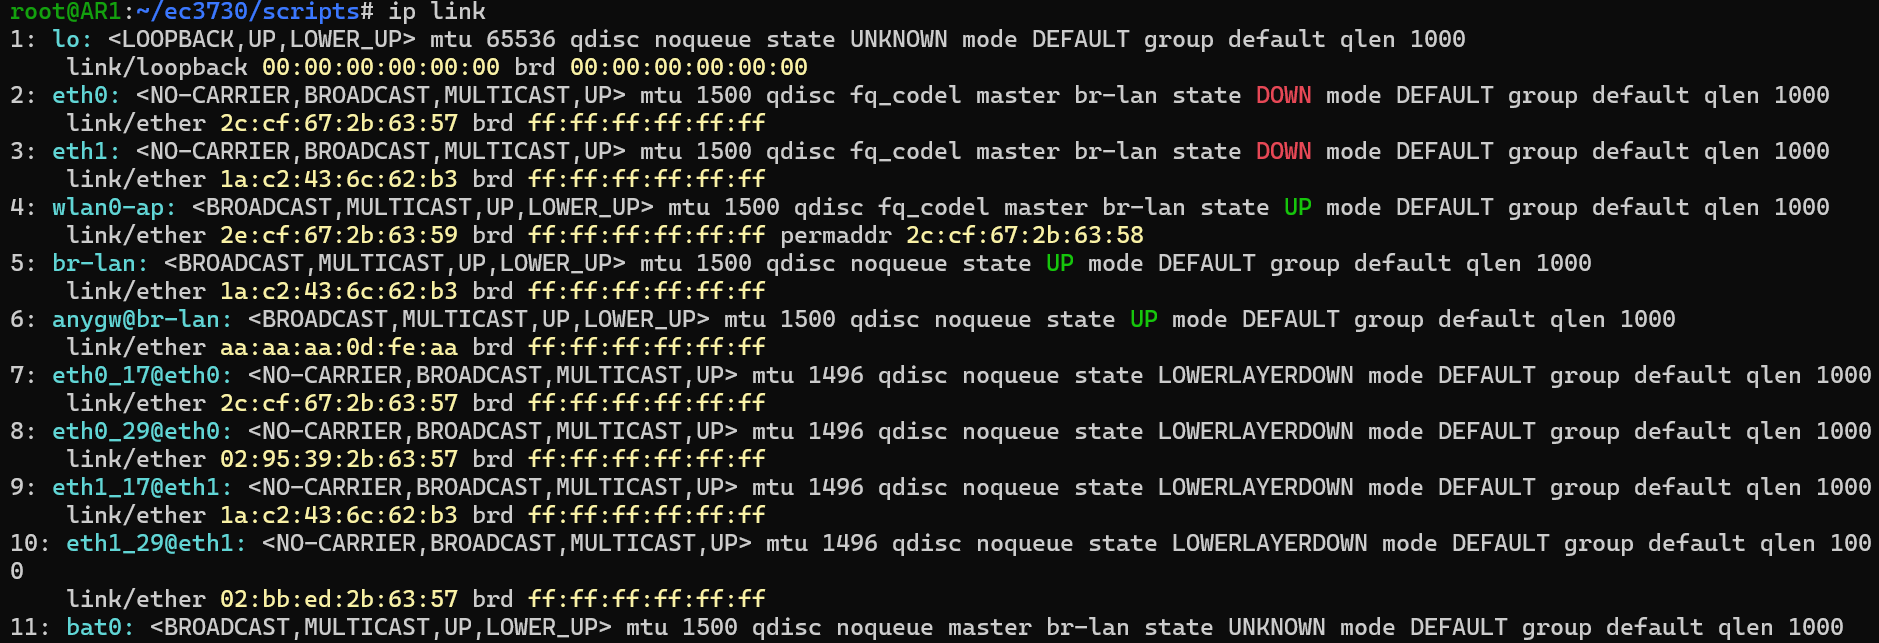
\includegraphics[width=\linewidth]{figures/ip-links.png}}
\caption{Wireless interface configuration and SSID verification.}
\label{fig:pi_wireless}
\end{figure}

This confirmed successful initialization of the onboard Raspberry Pi wireless hardware and demonstrated that the custom deployment parameters were correctly applied during image generation.

\subsubsection{BATMAN-adv Verification}

BATMAN-adv status commands were executed using:

\begin{verbatim}
batctl if
batctl n
batctl o
\end{verbatim}

At the time of testing, these commands produced no neighbor or originator entries.

This behavior was expected because only a single LibreMesh node had been deployed. BATMAN-adv requires multiple participating nodes before neighbor discovery and route propagation can occur.

The presence of the \texttt{bat0} interface nevertheless confirmed that BATMAN-adv had been loaded and initialized successfully.

\begin{figure}[htbp]
\centerline{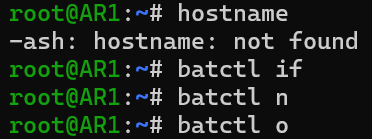
\includegraphics[width=\linewidth]{figures/batctl-req.png}}
\caption{BATMAN-adv verification commands executed on the Raspberry Pi node.}
\label{fig:pi_batctl}
\end{figure}

\subsubsection{LibreMesh Management Interface}

The LibreMesh management interface was accessed through a web browser using the node management address.

The management dashboard provided operational information including:

\begin{itemize}
    \item Device model
    \item Firmware version
    \item Network status
    \item Assigned addresses
    \item Routing information
\end{itemize}

\begin{figure}[htbp]
\centerline{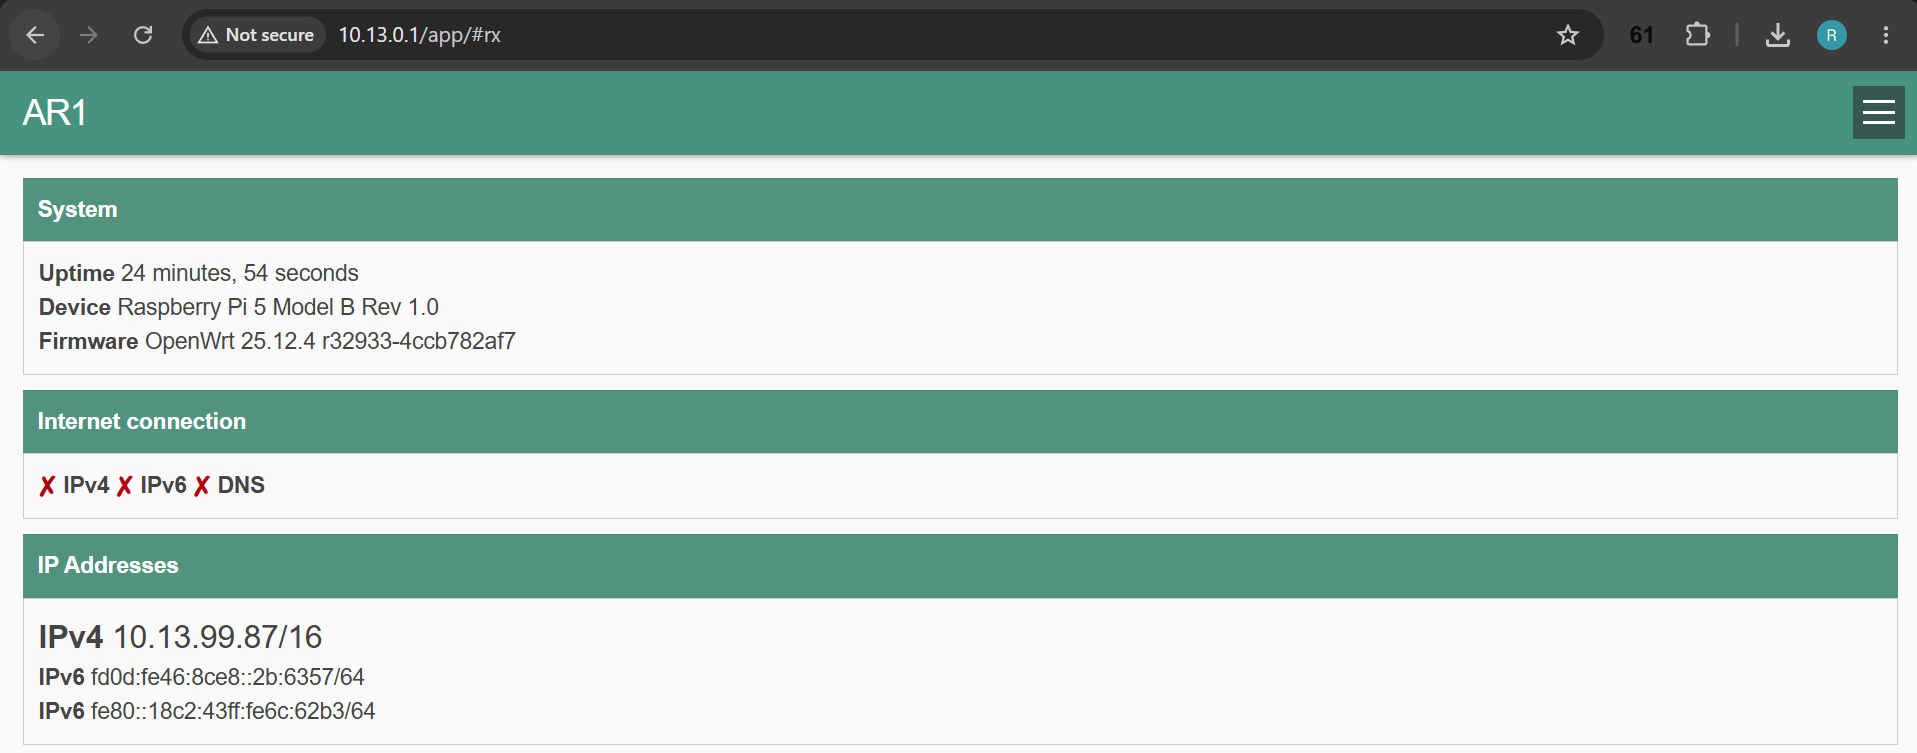
\includegraphics[width=\linewidth]{figures/lime-start-page.png}}
\caption{LibreMesh management dashboard running on Raspberry Pi 5.}
\label{fig:pi_limeapp}
\end{figure}

The successful operation of the management interface confirmed that the LibreMesh application framework, web services, and supporting middleware had been installed correctly.

Overall, the firmware exploration process demonstrated successful deployment of a customized LibreMesh image and verified that routing, wireless networking, management services, and BATMAN-adv components were operational prior to further mesh-network experimentation.

\subsection{Mesh Validation and Connectivity Verification}

Following deployment of two Raspberry Pi 5 nodes running LibreMesh, a series of connectivity tests were conducted to verify successful mesh formation and end-to-end communication. The nodes were interconnected using an Ethernet link configured as a BATMAN-adv transport interface. One Raspberry Pi hosted a wireless access point, while client devices including a laptop computer and smartphone connected to the network for testing.

Mesh operation was verified using BATMAN-adv diagnostic commands and Linux neighbor discovery tools. The command:

\begin{verbatim}
batctl meshif bat0 n
\end{verbatim}

confirmed successful neighbor discovery between the two mesh nodes, indicating that BATMAN-adv was exchanging routing information across the Ethernet transport.

Additional verification was performed using:

\begin{verbatim}
ip neigh
\end{verbatim}

which displayed dynamically learned neighboring devices throughout the mesh. The neighbor table contained entries corresponding to the participating Raspberry Pi nodes as well as connected client devices. These entries demonstrated that Layer 2 and Layer 3 communication was successfully propagating across the mesh infrastructure.

During testing, a smartphone was connected to the LibreMesh wireless network while a laptop computer maintained an SSH session into one of the Raspberry Pi nodes. The neighbor table showed reachable devices from multiple segments of the network, confirming successful forwarding of traffic through the mesh. ICMP testing further demonstrated successful communication between participating nodes.

These results confirmed that LibreMesh successfully established a functioning mesh topology using BATMAN-adv and automatically managed addressing within the 10.13.0.0/16 network space. The experiment validated neighbor discovery, route propagation, and client connectivity across the deployed mesh.

\begin{figure}[htbp]
\centerline{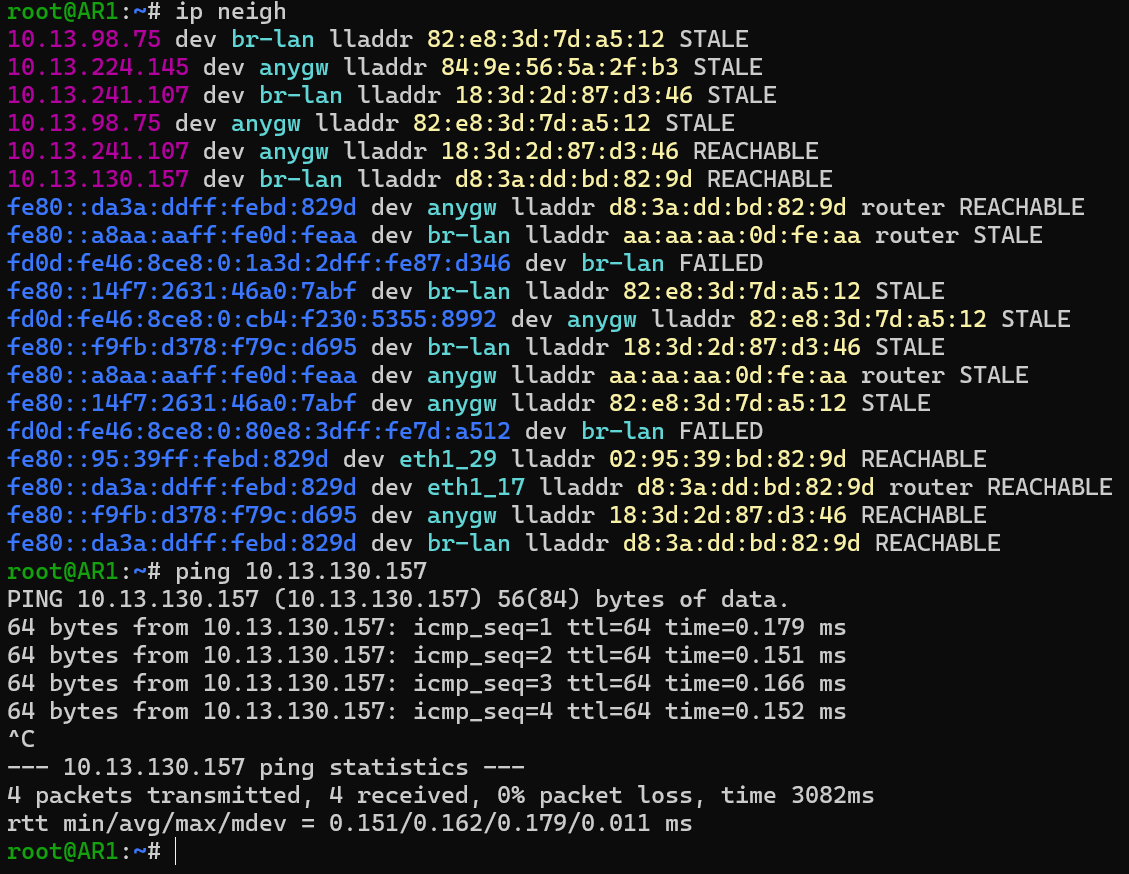
\includegraphics[width=\linewidth]{figures/ip-neigh-ping.png}}
\caption{Neighbor table showing dynamically learned devices within the LibreMesh deployment.}
\label{fig:mesh_validation}
\end{figure}
\begin{figure}[htbp]
\centerline{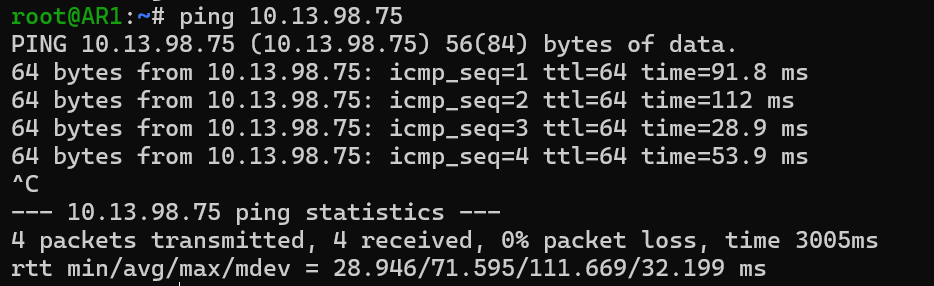
\includegraphics[width=\linewidth]{figures/ping-phone.png}}
\caption{Neighbor table showing dynamically learned devices within the LibreMesh deployment.}
\label{fig:mesh_validation}
\end{figure}

\subsection{Internet Gateway Deployment and Validation}

Following successful deployment of LibreMesh on Raspberry Pi 5 hardware, Internet gateway functionality was implemented using a dedicated Wide Area Network (WAN) interface. Initial attempts focused on providing Internet connectivity through wireless hotspot bridging; however, testing revealed that the Raspberry Pi 5 onboard wireless chipset could not reliably support simultaneous LibreMesh access point services, mesh functionality, and wireless client operation. As a result, a dedicated Ethernet-based gateway architecture was adopted.

The LibreMesh network configuration was modified to remove the second Ethernet interface (\texttt{eth1}) from the default bridge configuration. This interface was then reconfigured as a DHCP WAN interface and connected directly to an upstream residential router. Upon activation, the node successfully obtained an IP address from the upstream network and installed a default route to the Internet.

A simplified topology of the resulting configuration is shown below:

\begin{verbatim}
Internet
|
Home Router
|
eth1 (WAN)
|
AR1
|
BATMAN-adv / LibreMesh
|
Wireless and Mesh Clients
\end{verbatim}

Verification of Internet connectivity was performed using standard network diagnostic tools. The node successfully acquired the address \texttt{192.168.1.235} from the upstream router and established a default route through gateway \texttt{192.168.1.254}. Connectivity was confirmed by successfully pinging external Internet hosts, including Google's public DNS server (\texttt{8.8.8.8}).

LibreMesh AnyGW functionality was then enabled by configuring BATMAN-adv gateway mode as a server. Verification using BATMAN diagnostic tools confirmed that the node was advertising gateway services to participating mesh nodes.

To validate end-user connectivity, an Apple iPhone was connected to the LibreMesh wireless access point (\texttt{EC3730}). The device successfully received a LibreMesh network address within the mesh subnet and was able to access external Internet resources through the gateway node. Client association was verified using wireless station monitoring tools, while routing behavior was confirmed through neighbor table inspection and Internet connectivity testing.

This experiment demonstrated successful integration of LibreMesh routing, BATMAN-adv gateway services, wireless client access, and upstream Internet connectivity on physical Raspberry Pi hardware. The resulting configuration establishes the foundation required for future AnyGW testing involving multiple interconnected mesh nodes and automatic gateway discovery across the mesh network.

\begin{figure}[htbp]
\centerline{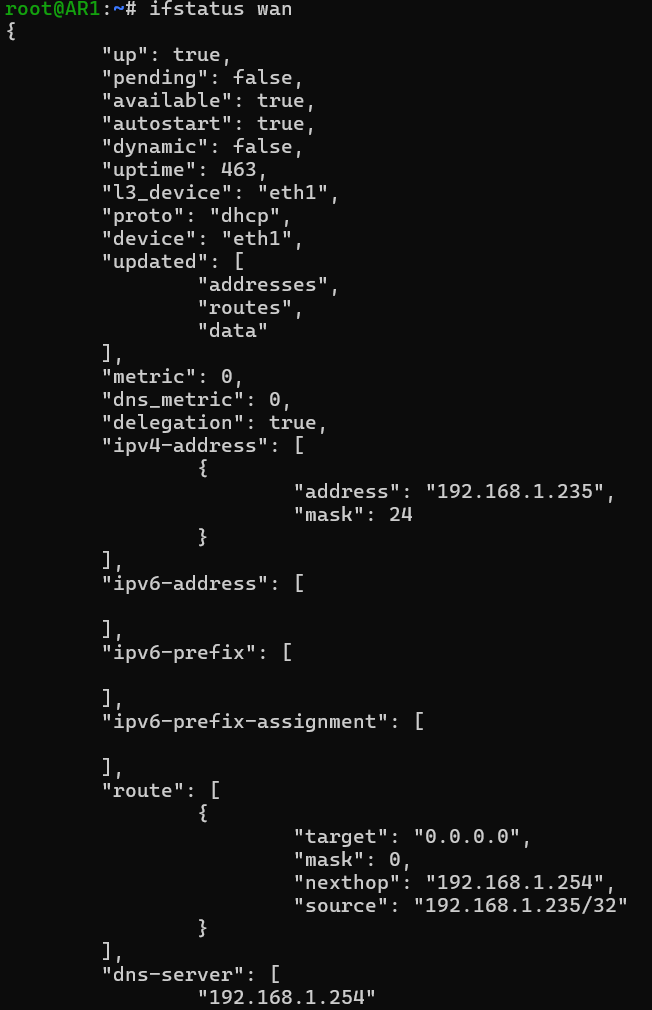
\includegraphics[width=\linewidth]{figures/ifstatus_wan1.png}}
\caption{WAN interface successfully obtaining a DHCP address from the upstream router.}
\label{fig:wan_dhcp}
\end{figure}
\begin{figure}[htbp]
\centerline{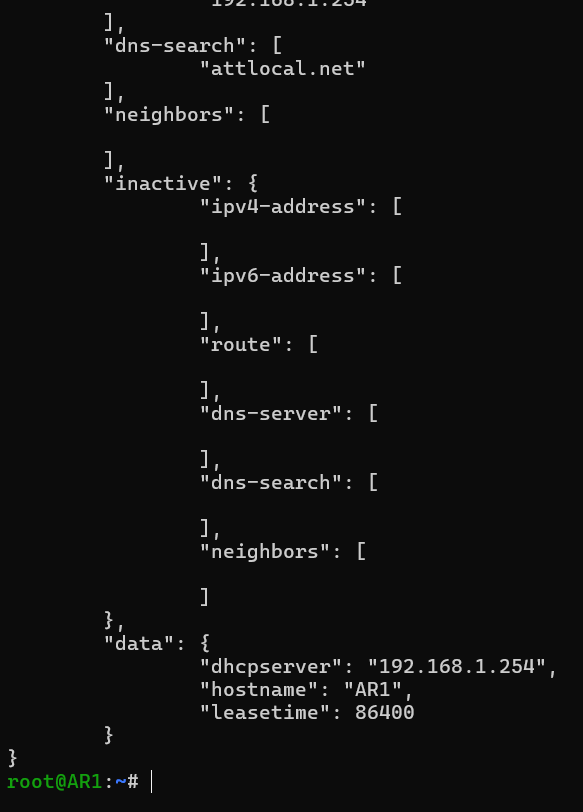
\includegraphics[width=\linewidth]{figures/ifstatus_wan2.png}}
\caption{WAN interface successfully obtaining a DHCP address from the upstream router.}
\label{fig:wan_dhcp2}
\end{figure}

\begin{figure}[htbp]
\centerline{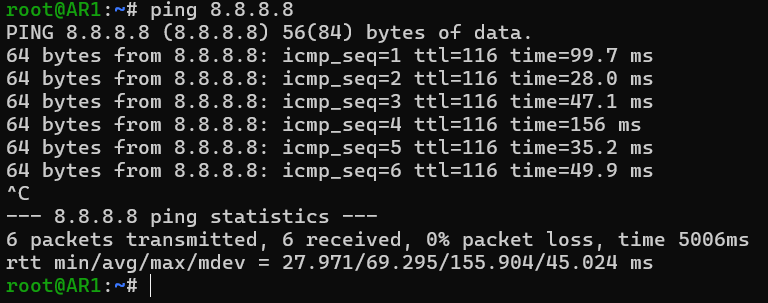
\includegraphics[width=\linewidth]{figures/ping_8_8_8_8.png}}
\caption{Successful Internet connectivity verification from the LibreMesh gateway node.}
\label{fig:internet_ping}
\end{figure}

\begin{figure}[htbp]
\centerline{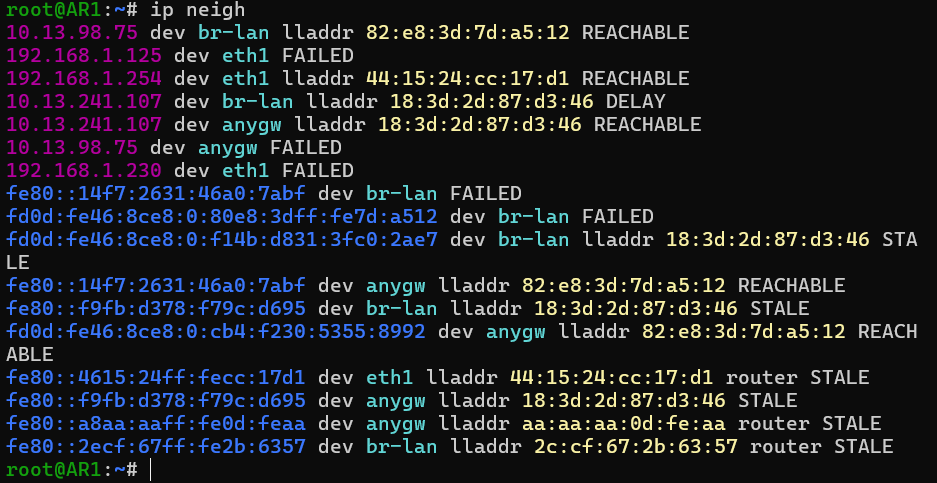
\includegraphics[width=\linewidth]{figures/ip_neigh_phone_connected.png}}
\caption{Neighbor table showing a wireless client connected to the LibreMesh access point and participating in the mesh network.}
\label{fig:phone_connected}
\end{figure}

\begin{figure}[htbp]
\centerline{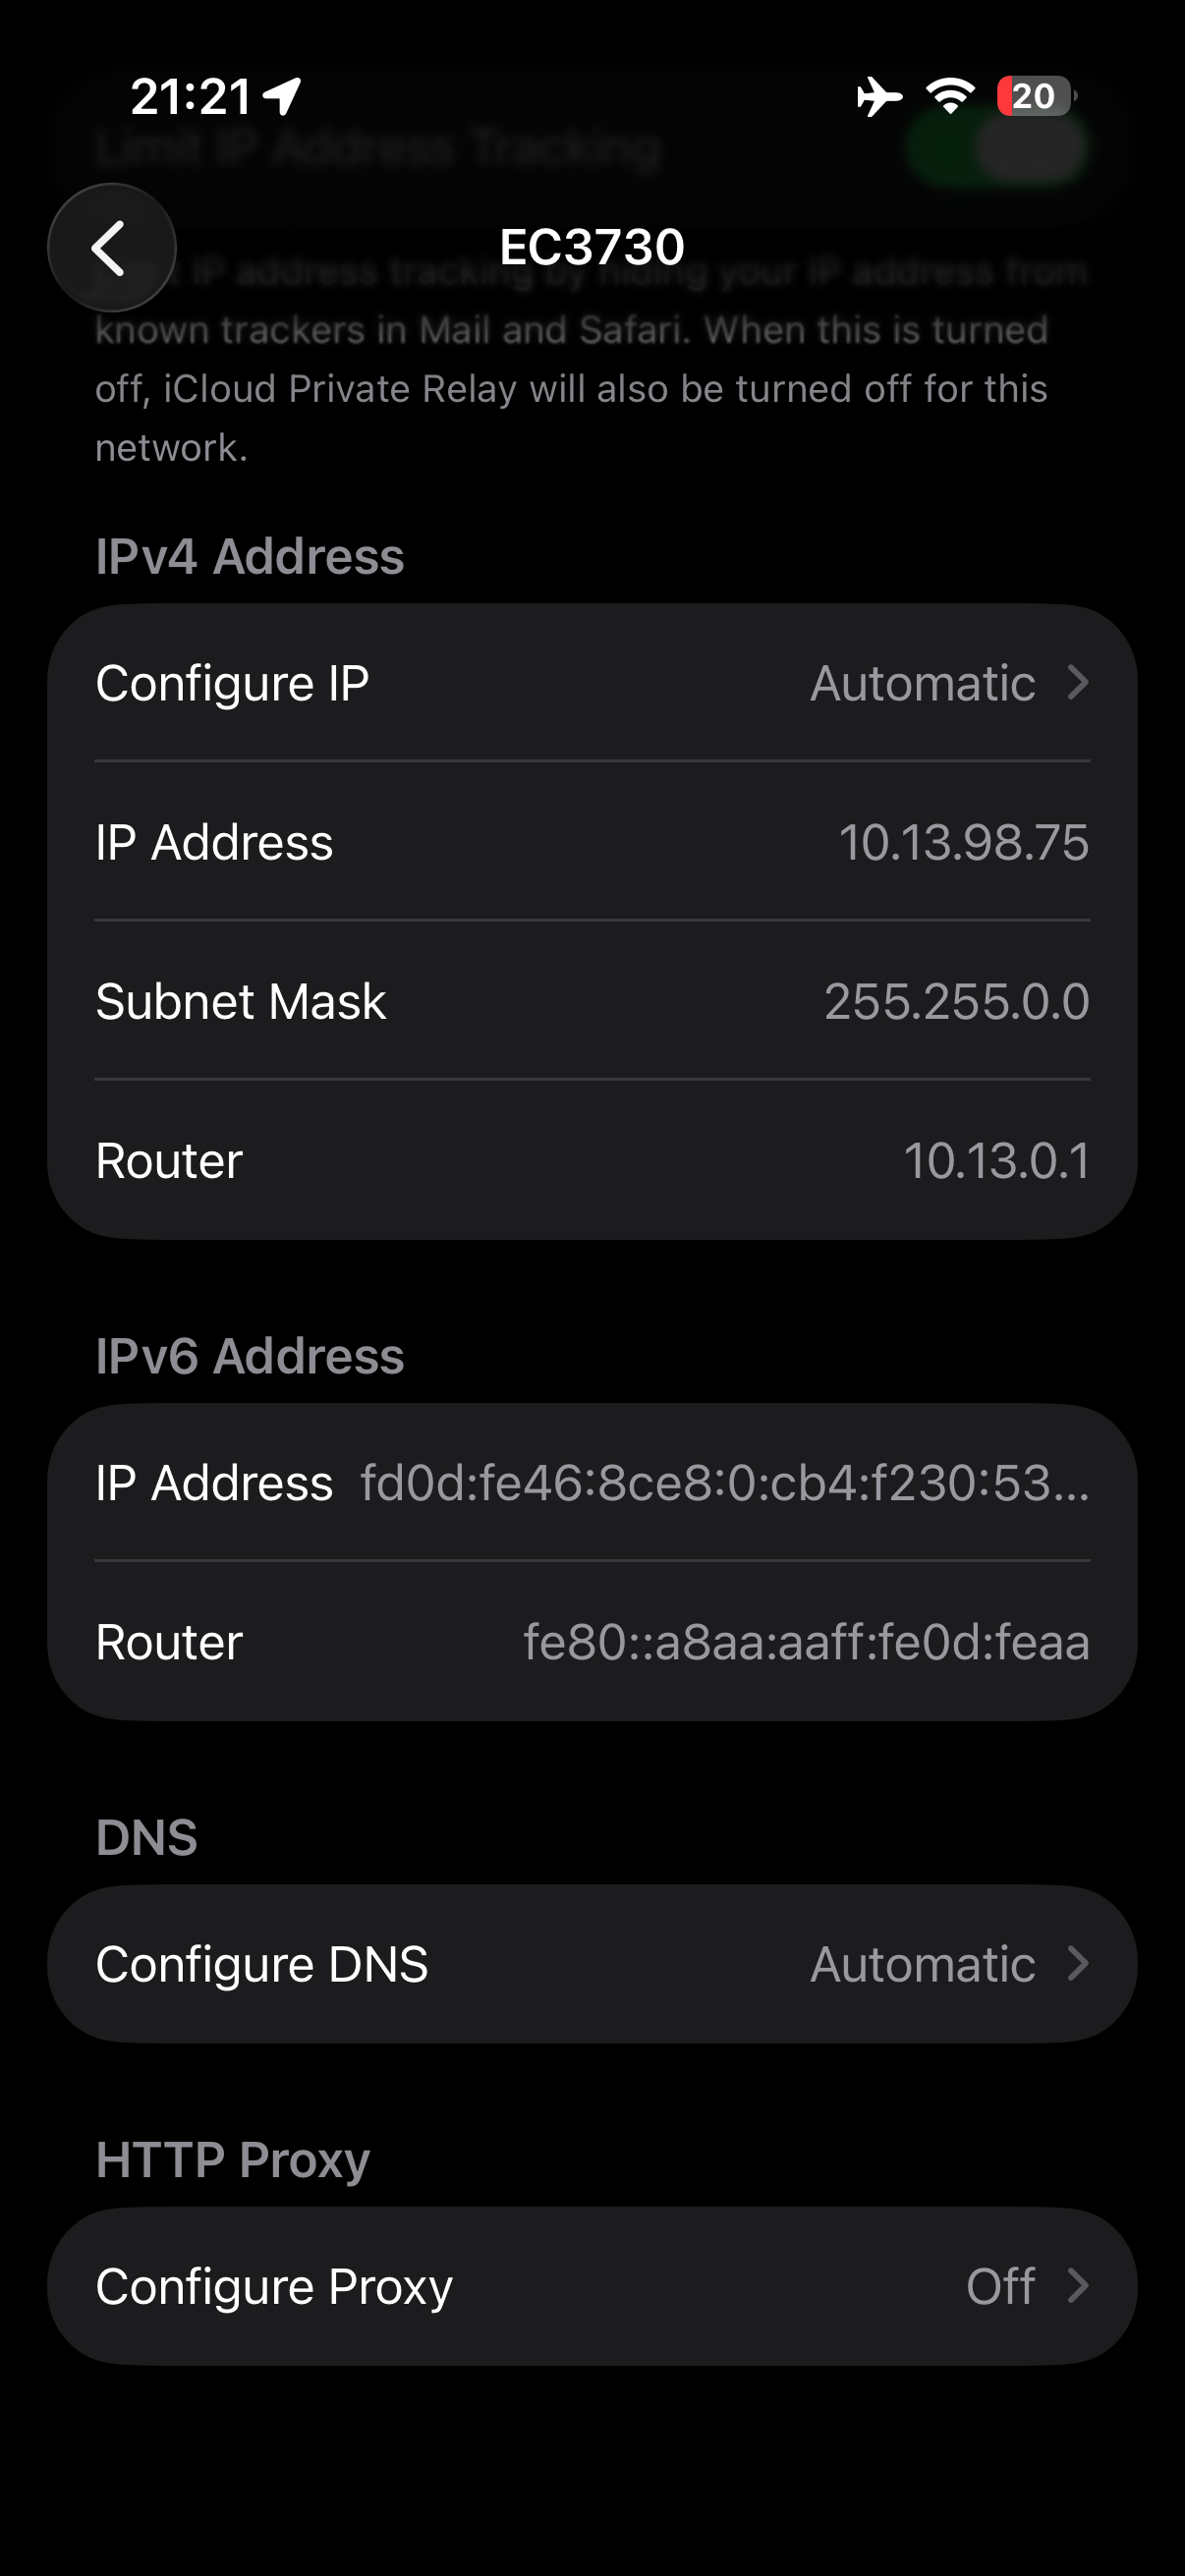
\includegraphics[width=\linewidth]{figures/ip_neigh_phone_connected_phone.png}}
\caption{Neighbor table showing a wireless client connected to the LibreMesh access point and participating in the mesh network.}
\label{fig:phone_connected_phone}
\end{figure}

\subsection{Wireless Mesh Interface Investigation and Hardware Limitations}

During testing, an effort was made to utilize LibreMesh's native IEEE 802.11s wireless mesh functionality on Raspberry Pi 5 hardware. LibreMesh automatically generated a wireless mesh interface (\texttt{wlan0-mesh}) and associated BATMAN-adv configuration; however, the interface repeatedly failed to become operational despite appearing correctly configured within OpenWrt.

Several troubleshooting procedures were performed, including verification of wireless configuration files, inspection of kernel logs, interface status monitoring, and testing of simultaneous wireless access point and client operation. Although the mesh interface was present within the LibreMesh configuration, diagnostic commands consistently showed that the interface was unable to successfully initialize. Kernel logs repeatedly reported interface activation failures and MTU-related errors during wireless mesh initialization.

Further investigation was conducted using the command:

\begin{verbatim}
iw phy phy0 info
\end{verbatim}

which revealed the wireless capabilities supported by the Raspberry Pi 5 onboard Broadcom wireless chipset. The supported interface modes included:

\begin{itemize}
\item Managed (Client)
\item Access Point (AP)
\item IBSS (Ad-Hoc)
\item Peer-to-Peer (P2P)
\end{itemize}

However, the wireless driver did not advertise support for the IEEE 802.11s \texttt{mesh point} interface mode required for native wireless mesh networking. As a result, LibreMesh was unable to establish a functional wireless mesh interface despite generating the appropriate configuration.

These findings suggest that the limitation originates from the Broadcom \texttt{brcmfmac} driver and associated firmware rather than from LibreMesh itself. While wireless access point functionality operated correctly and BATMAN-adv routing functioned successfully over Ethernet links, native wireless mesh operation could not be validated on the Raspberry Pi 5 platform using the onboard wireless hardware.

Consequently, all successful mesh-network testing performed during this project utilized BATMAN-adv over Ethernet transport links between Raspberry Pi nodes. Wireless connectivity remained available for client devices through the LibreMesh access point service, allowing smartphones, laptops, and other devices to access the mesh network while routing functions were performed through wired backbone connections.

Future work may investigate the use of external USB wireless adapters with confirmed IEEE 802.11s support, alternative OpenWrt-compatible hardware platforms, or updated wireless drivers that provide native mesh-point functionality.

\begin{figure}[htbp]
\centerline{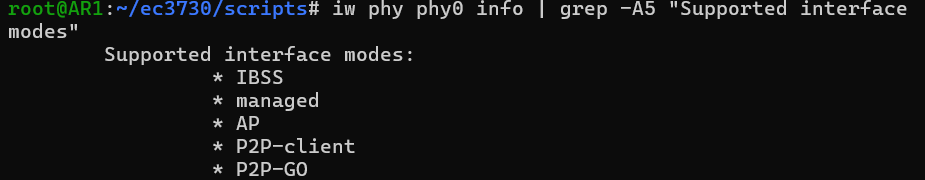
\includegraphics[width=\linewidth]{figures/iw_phy_supported_modes.png}}
\caption{Supported wireless interface modes reported by the Raspberry Pi 5 Broadcom wireless chipset. The absence of IEEE 802.11s mesh-point support prevented native wireless mesh operation.}
\label{fig:iw_phy_modes}
\end{figure}

\subsection{Demonstration Plan and Presentation Validation}

A live demonstration is planned to validate the physical LibreMesh deployment and illustrate mesh-network operation using two Raspberry Pi 5 nodes configured with LibreMesh firmware. The two nodes will be interconnected using an Ethernet backbone connection through their mesh interfaces, allowing BATMAN-adv to establish neighbor relationships and exchange routing information.

One Raspberry Pi will be configured as an Internet gateway node. The gateway node will utilize a dedicated WAN interface connected to a laptop computer. The laptop will obtain Internet connectivity through a mobile hotspot connection and provide upstream network access to the LibreMesh node through Ethernet. This configuration will allow the LibreMesh gateway to distribute Internet access throughout the mesh network using LibreMesh AnyGW services.

A simplified demonstration topology is shown below:

\begin{verbatim}
Mobile Hotspot
|
Laptop
|
Ethernet
|
AR1 (Gateway)
|
BATMAN-adv Mesh
|
BR1 Node
|
Wireless Clients
\end{verbatim}

Audience members will be invited to join the EC3730 wireless network using smartphones, tablets, and laptop computers. Devices connected to the wireless network will receive LibreMesh IP addresses and gain access to both local mesh resources and external Internet connectivity through the gateway node.

The demonstration will focus on four primary validation activities:

\begin{enumerate}

\item Verification of BATMAN-adv neighbor discovery using:

\begin{verbatim}
batctl n
\end{verbatim}

This command will display neighboring mesh nodes and confirm successful Layer 2 mesh formation across the Ethernet backbone.

\item Verification of route propagation and originator advertisements using:

\begin{verbatim}
batctl o
\end{verbatim}

The originator table will demonstrate that routing information is being exchanged between mesh participants and that BATMAN-adv has established valid forwarding paths.

\item Verification of connected clients using:

\begin{verbatim}
ip neigh
iw dev wlan0-ap station dump
\end{verbatim}

These commands will display client devices currently participating in the mesh network and verify successful wireless association with the LibreMesh access point.

\item Verification of Internet connectivity and end-to-end communication.

Connected users will be instructed to access Internet resources and perform ICMP connectivity tests. Participants will ping external hosts such as Google's public DNS server (\texttt{8.8.8.8}) and communicate with other connected devices to demonstrate successful routing through the mesh infrastructure.

\end{enumerate}

Successful completion of these tests will demonstrate operation of LibreMesh services, BATMAN-adv routing, AnyGW gateway functionality, wireless client access, and Internet connectivity within a physical mesh-network deployment. The presentation will provide a practical example of decentralized networking principles and illustrate how community mesh networks can distribute connectivity across multiple nodes while maintaining access to external network resources.


\section{Unresolved Operational Challenges and Future Investigation}

Although the distributed BATMAN-adv mesh deployment operated successfully overall, several operational inconsistencies and unresolved behaviors were identified during experimentation.

These issues represent valuable future investigation areas for both virtualized and physical mesh deployments.

\subsection{Persistent VMware DHCP Address Duplication}

Although earlier sequential startup procedures improved DHCP convergence behavior, VMware NAT services still occasionally assigned identical WAN-side addresses to multiple cloned OpenWrt nodes.

Example observed behavior included:

\begin{itemize}
    \item Multiple nodes simultaneously assigned 192.168.111.141
    \item Ambiguous SSH access
    \item Non-deterministic LuCI management behavior
    \item Administrative-plane collisions
\end{itemize}

Although sequential startup reduced the frequency of collisions, duplicate assignments still occasionally reappeared during extended experimentation.

The issue appeared isolated to VMware NAT-side DHCP behavior and did not affect BATMAN forwarding functionality operating on the dedicated mesh backbone interface.

This behavior represents an important virtualization-management limitation requiring further investigation.

\subsection{IPv6 Duplicate Address Detection Events}

OpenWrt repeatedly reported IPv6 duplicate address detection warnings during sequential startup and node cloning operations:

\begin{lstlisting}
IPv6 duplicate address detected
\end{lstlisting}

Despite repeated warnings:

\begin{itemize}
    \item IPv4 routing remained operational
    \item BATMAN mesh convergence persisted
    \item Node-to-node communication remained stable
\end{itemize}

The project did not fully investigate:

\begin{itemize}
    \item IPv6 address autoconfiguration behavior
    \item Duplicate IPv6 neighbor advertisements
    \item IPv6 interactions with BATMAN-adv
    \item Potential virtualization-layer MAC/address reuse
\end{itemize}

Future work should evaluate whether disabling IPv6 entirely or implementing static IPv6 addressing would improve deployment stability.

\subsection{Management-Plane and Forwarding-Plane Separation}

The project revealed significant architectural separation between:

\begin{itemize}
    \item Administrative management-plane behavior
    \item BATMAN distributed forwarding behavior
\end{itemize}

Even during severe management-plane inconsistencies:

\begin{itemize}
    \item BATMAN neighbor discovery remained stable
    \item Originator propagation continued
    \item Distributed forwarding functionality persisted
\end{itemize}

This behavior further confirmed the resilience of BATMAN forwarding despite administrative-plane instability.

\subsection{Lightweight Embedded Linux Limitations}

Several OpenWrt operational limitations were identified during experimentation:

\begin{itemize}
    \item Missing HTTPS support in BusyBox wget
    \item Missing SFTP subsystem support in Dropbear
    \item Minimal shell-tool availability
    \item CRLF/LF shell-script compatibility issues
\end{itemize}

These limitations complicated:
\begin{itemize}
    \item Package installation
    \item Secure artifact transfer
    \item Deployment automation
    \item Remote administration
\end{itemize}

While expected for lightweight embedded environments, these limitations introduced significant operational overhead during deployment and experimentation.

\subsection{Incomplete Multi-Hop Routing Validation}

Although the BATMAN mesh operated successfully across all four nodes, the VMware host-only topology allowed all routers to remain directly adjacent at Layer 2.

As a result, the deployment did not fully validate:

\begin{itemize}
    \item True multi-hop relay behavior
    \item Intermediate-node forwarding dependency
    \item Mesh partition recovery
    \item Indirect route optimization
\end{itemize}

Future work should intentionally isolate subsets of nodes to force multi-hop forwarding paths and evaluate true relay-based mesh behavior.

\subsection{Future WireGuard-Based Inter-Mesh Federation}

Future experimentation may connect independent BATMAN mesh deployments between project groups using encrypted WireGuard overlay tunnels.

Potential future architecture:

\begin{itemize}
    \item Independent local BATMAN clusters
    \item WireGuard encrypted Internet overlays
    \item Distributed inter-group route propagation
    \item Geographically separated mesh federation
\end{itemize}

This would allow evaluation of:
\begin{itemize}
    \item Distributed mesh scalability
    \item Internet-based overlay transport
    \item Secure inter-cluster communication
    \item Hybrid mesh-overlay architectures
\end{itemize}

\section{Conclusion}

This project successfully implemented a persistent four-node distributed OpenWrt mesh-routing laboratory environment using VMware virtualization and BATMAN-adv.

The completed deployment demonstrated:

\begin{itemize}
    \item Successful OpenWrt virtualization
    \item Stable multi-node routed mesh backbone construction
    \item Autonomous BATMAN neighbor discovery
    \item Dynamic distributed originator propagation
    \item Persistent mesh deployment through UCI configuration
    \item Autonomous reconvergence after node failure
    \item BATMAN-native ping and traceroute functionality
    \item MTU optimization and fragmentation analysis
    \item Packet-level mesh observation using tcpdump
    \item Identification of virtualization and management-plane edge cases
\end{itemize}

The project evolved significantly beyond initial router virtualization objectives and ultimately produced a functional distributed autonomous mesh-routing research platform suitable for continued LibreMesh experimentation and future Raspberry Pi deployment.

The completed environment represents a robust foundation for continued experimentation with decentralized community-networking infrastructure using LibreMesh and BATMAN-adv.

\subsection{Post Presentation Conclusion}

This project successfully implemented and evaluated LibreMesh and BATMAN-adv in both virtualized and physical deployment environments. Initial experimentation was conducted using a four-node OpenWrt mesh laboratory hosted within VMware, providing a controlled environment for studying decentralized routing behavior, fault tolerance, route propagation, and mesh-network management. The project was subsequently extended to physical Raspberry Pi 5 hardware, where LibreMesh was deployed and validated using real wireless clients and Internet gateway services.

The completed deployment demonstrated successful OpenWrt virtualization, BATMAN-adv mesh formation, autonomous neighbor discovery, dynamic route propagation, persistent configuration management through UCI, and recovery from topology changes. Additional testing validated wireless client connectivity, Internet gateway functionality, and operation of LibreMesh AnyGW services. A dedicated WAN interface was successfully implemented on a Raspberry Pi node, allowing Internet connectivity to be distributed to wireless clients connected through the mesh network.

A key outcome of this project was understanding the interaction between multiple routing technologies within LibreMesh. BATMAN-adv operates primarily as a Layer 2 mesh-routing protocol, creating a virtual distributed Ethernet segment across participating nodes. Unlike traditional routing protocols such as OSPF, BATMAN-adv does not maintain a complete network topology database or compute shortest paths using Dijkstra's algorithm. Instead, nodes exchange Originator Messages (OGMs) and determine only the best next-hop neighbor toward each destination. This approach reduces routing overhead and improves adaptability in dynamic mesh environments.

LibreMesh additionally incorporates the Babel routing protocol, which operates at Layer 3 and is responsible for exchanging IP routing information between nodes. While BATMAN-adv provides distributed Layer 2 connectivity, Babel contributes Layer 3 route dissemination and network reachability information. Together, these protocols provide a hybrid architecture that combines Layer 2 mesh forwarding with Layer 3 routing intelligence.

Internet gateway distribution is facilitated through LibreMesh AnyGW functionality. AnyGW allows nodes possessing Internet connectivity to advertise gateway services throughout the mesh. Other mesh participants may automatically discover and utilize available gateways without requiring manual route configuration. Testing demonstrated successful operation of a gateway-enabled Raspberry Pi node and validated Internet access from wireless client devices connected to the mesh.

The project also revealed several practical implementation considerations. Configuration files stored by OpenWrt and LibreMesh maintain wireless SSIDs and pre-shared keys in plain-text format within system configuration files rather than storing only cryptographic hashes. While this simplifies administration and automated deployment, it also highlights the importance of securing administrative access to mesh nodes and protecting configuration backups from unauthorized disclosure.

Overall, the completed environment represents a functional distributed mesh-networking platform suitable for continued experimentation with decentralized community networking, Internet gateway distribution, routing protocol analysis, and future extensions involving WireGuard integration, larger mesh deployments, and advanced LibreMesh services. The project successfully demonstrated both the theoretical and practical aspects of modern mesh networking and established a robust foundation for future research and development.


\bibliographystyle{IEEEtran}

\begin{thebibliography}{99}

\bibitem{openwrt}
OpenWrt Project, ``OpenWrt Documentation,'' [Online]. Available: \url{https://openwrt.org}

\bibitem{libremesh}
LibreMesh Project, ``LibreMesh Documentation,'' [Online]. Available: \url{https://libremesh.org}

\bibitem{bmx7}
BMX7 Routing Protocol, ``BMX7 GitHub Repository,'' [Online]. Available: \url{https://github.com/bmx-routing/bmx7}

\bibitem{batmanadv}
BATMAN-adv Project, ``B.A.T.M.A.N. advanced Documentation,'' [Online]. Available: \url{https://www.open-mesh.org/projects/batman-adv/wiki}

\bibitem{batctl}
Open-Mesh, ``batctl User Guide,'' [Online]. Available: \url{https://www.open-mesh.org/projects/batman-adv/wiki/Batctl}

\bibitem{vmware}
VMware Inc., ``VMware Workstation Pro Documentation,'' [Online]. Available: \url{https://docs.vmware.com}

\bibitem{chatgpt}
OpenAI, ``ChatGPT,'' [Online]. Available: \url{https://chat.openai.com}

\bibitem{libremeshdocs}
LibreMesh Project, ``LibreMesh Documentation,'' [Online]. Available: \url{https://libremesh.org}

\bibitem{libremeshgettingstarted}
LibreMesh Project, ``Getting Started,'' [Online]. Available: \url{https://libremesh.org/getting-started.html}

\bibitem{libremeshprotocols}
LibreMesh Project, ``Network Protocol Options,'' [Online]. Available: \url{https://libremesh.org/reference/network/protocols-options.html}

\bibitem{limerouteredt}
Earth Defenders Toolkit, ``Guide: LibreRouter and LibreMesh,'' [Online]. Available: \url{https://www.earthdefenderstoolkit.com/one-pager/guide-librerouter-and-libremesh/}

\bibitem{batmanadvdocs}
BATMAN-adv Project, ``B.A.T.M.A.N. advanced Documentation,'' [Online]. Available: \url{https://www.open-mesh.org/doc/batman-adv/Wiki.html}

\bibitem{openwrtbatman}
OpenWrt Project, ``B.A.T.M.A.N. / batman-adv,'' [Online]. Available: \url{https://openwrt.org/docs/guide-user/network/wifi/mesh/batman}

\bibitem{openwrtsecurity}
OpenWrt Project, ``Security,'' [Online]. Available: \url{https://openwrt.org/docs/guide-developer/security}

\bibitem{openwrtsigissue}
OpenWrt Project, ``opkg update Signature check failed for luci,'' GitHub Issue, [Online]. Available: \url{https://github.com/openwrt/openwrt/issues/19316}

\bibitem{guifinetcommons}
R. Baig, R. Roca, F. Freitag, and L. Navarro, ``guifi.net, a crowdsourced network infrastructure held in common,'' Computer Networks, 2015.

\bibitem{guifinetexperimental}
L. Cerda-Alabern, ``Experimental Evaluation of a Wireless Community Mesh Network,'' [Online]. Available: \url{https://pdfs.semanticscholar.org/e18f/9cff9dab586d63c54149014ec99f2eaea134.pdf}

\bibitem{gluon}
Gluon Project, ``Welcome to Gluon,'' [Online]. Available: \url{https://gluon.readthedocs.io/}

\bibitem{nycmeshcase}
Resilient Comms, ``NYC Mesh: Community Internet Infrastructure,'' [Online]. Available: \url{https://resilientcomms.org/case-studies/nyc-mesh-community-network}

\bibitem{wmnsecurity}
IEEE Denver, ``Securing Wireless Mesh Networks,'' [Online]. Available: \url{https://ieee-denver.org/wp-content/uploads/sites/23/2022/10/Securing_Wireless_Mesh_Networks-1.pdf}

\bibitem{commotionaudit}
Open Technology Fund, ``Commotion Android Security Audit,'' [Online]. Available: \url{https://www.opentech.fund/security-safety-audits/commotion-android/}

\bibitem{libremesh_anygw}
LibreMesh Project,
\textit{Network Protocol Options},
Available: \url{https://libremesh.org/reference/network/protocols-options.html}
Accessed: May 2026.

\bibitem{libremesh_howitworks}
LibreMesh Project,
\textit{How LibreMesh Works},
Available: \url{https://www.onnocenter.or.id/wiki/index.php/LibreMesh:_How_It_Works}
Accessed: May 2026.

\end{thebibliography}

\section*{AI Usage Disclosure}

Artificial intelligence tools were used during portions of this project to assist with:

\begin{itemize}
    \item Technical troubleshooting
    \item Linux and OpenWrt command analysis
    \item BATMAN-adv deployment guidance
    \item VMware networking diagnostics
    \item LaTeX report formatting
    \item Documentation organization and editing
\end{itemize}

AI-assisted guidance was used interactively throughout deployment and experimentation; however, all configuration, implementation, troubleshooting, validation, testing, and analysis were performed directly by the project team.

The report content was reviewed, modified, and validated manually to ensure technical accuracy and consistency with observed system behavior.

OpenAI ChatGPT was used as an engineering-assistance and documentation-support tool during the project lifecycle.

\appendices

\section{Exported Configuration and Operational Artifacts}

The following exported artifacts were generated and archived from each OpenWrt node:

\begin{itemize}
    \item network-nodeX
    \item system-nodeX
    \item firewall-nodeX
    \item dhcp-nodeX
    \item batman-if-nodeX.txt
    \item batman-neighbors-nodeX.txt
    \item batman-originators-nodeX.txt
    \item ip-addr-nodeX.txt
    \item ip-route-nodeX.txt
    \item packages-nodeX.txt
\end{itemize}

These artifacts provide reproducible deployment state information and operational validation for the completed distributed BATMAN-adv mesh environment.

\appendix

\section{Command Reference}

This appendix documents the primary commands used throughout the project during virtual machine development, Git repository management, LibreMesh deployment, BATMAN-adv configuration, AnyGW implementation, and system validation.

\subsection{VMware and Windows Commands}

\subsubsection{Network Configuration}

\paragraph{Display Network Configuration}
\begin{verbatim}
ipconfig
\end{verbatim}
Displays the IP configuration of all network adapters including IPv4 addresses, subnet masks, and default gateways.

\paragraph{Display Detailed Network Configuration}
\begin{verbatim}
ipconfig /all
\end{verbatim}
Displays detailed information about all network adapters, including MAC addresses, DHCP information, DNS servers, and lease information.

\paragraph{Ping a Device}
\begin{verbatim}
ping <IP Address>
\end{verbatim}
Tests network connectivity to another device by sending ICMP echo requests.

Example:
\begin{verbatim}
ping 10.13.99.87
\end{verbatim}

\paragraph{Display ARP Table}
\begin{verbatim}
arp -a
\end{verbatim}
Displays the Address Resolution Protocol (ARP) cache showing IP-to-MAC address mappings.

\subsubsection{SSH Connectivity}

\paragraph{Connect to a LibreMesh Node}
\begin{verbatim}
ssh root@<IP Address>
\end{verbatim}
Creates a secure shell connection to a LibreMesh node.

Example:
\begin{verbatim}
ssh root@10.13.99.87
\end{verbatim}

\subsubsection{Git Repository Management}

\paragraph{Check Repository Status}
\begin{verbatim}
git status
\end{verbatim}
Displays modified, staged, and untracked files.

\paragraph{Add All Files}
\begin{verbatim}
git add .
\end{verbatim}
Stages all modified files for commit.

\paragraph{Create Commit}
\begin{verbatim}
git commit -m "Commit Message"
\end{verbatim}
Creates a snapshot of the repository changes.

\paragraph{Upload Changes}
\begin{verbatim}
git push
\end{verbatim}
Uploads local commits to the remote repository.

\paragraph{Clone Repository}
\begin{verbatim}
git clone <repository-url>
\end{verbatim}
Downloads a repository from a remote source.

\paragraph{Pull Updates}
\begin{verbatim}
git pull
\end{verbatim}
Downloads and merges updates from the remote repository.

\paragraph{Remove Cached File}
\begin{verbatim}
git rm --cached <filename>
\end{verbatim}
Removes a file from Git tracking while keeping the local copy.

\paragraph{Remove All Cached Files}
\begin{verbatim}
git rm -r --cached .
\end{verbatim}
Removes all files from Git tracking without deleting local copies.

\subsection{Raspberry Pi and LibreMesh Commands}

\subsubsection{Wireless Configuration}

\paragraph{Display Wireless Configuration}
\begin{verbatim}
uci show wireless
\end{verbatim}
Displays all wireless settings stored in OpenWrt.

\paragraph{Display Wireless Interfaces}
\begin{verbatim}
iw dev
\end{verbatim}
Displays all wireless interfaces and operating modes.

\paragraph{Display Wireless Information}
\begin{verbatim}
iwinfo
\end{verbatim}
Displays SSID, channel, encryption, signal levels, and interface status.

\paragraph{Scan Nearby Wireless Networks}
\begin{verbatim}
iw dev wlan0-mesh scan | grep SSID
\end{verbatim}
Scans for nearby wireless networks and displays detected SSIDs.

\paragraph{Reload Wireless Configuration}
\begin{verbatim}
wifi reload
\end{verbatim}
Applies wireless configuration changes without requiring a reboot.

\subsubsection{Network Configuration}

\paragraph{Display Network Configuration}
\begin{verbatim}
uci show network
\end{verbatim}
Displays all OpenWrt network settings.

\paragraph{Display Interface Status}
\begin{verbatim}
ifstatus <interface>
\end{verbatim}
Displays operational information about a network interface.

Examples:
\begin{verbatim}
ifstatus wan
ifstatus wwan
\end{verbatim}

\paragraph{Display IP Addresses}
\begin{verbatim}
ip addr
\end{verbatim}
Shows all network interfaces and assigned IP addresses.

\paragraph{Display Routing Table}
\begin{verbatim}
ip route
\end{verbatim}
Displays the kernel routing table.

\paragraph{Display Neighbor Table}
\begin{verbatim}
ip neigh
\end{verbatim}
Displays neighboring devices discovered through ARP and IPv6 Neighbor Discovery.

\paragraph{Restart Networking}
\begin{verbatim}
/etc/init.d/network restart
\end{verbatim}
Restarts all OpenWrt networking services.

\subsubsection{UCI Configuration Commands}

\paragraph{Read Configuration Value}
\begin{verbatim}
uci get <option>
\end{verbatim}
Displays the current value of a configuration option.

Example:
\begin{verbatim}
uci get network.bat0.gw_mode
\end{verbatim}

\paragraph{Modify Configuration}
\begin{verbatim}
uci set <option>=<value>
\end{verbatim}
Changes a configuration setting.

Example:
\begin{verbatim}
uci set wireless.lm_wlan0_ap_radio0.ssid='EC3730A'
\end{verbatim}

\paragraph{Delete Configuration Entry}
\begin{verbatim}
uci delete <section>
\end{verbatim}
Removes a configuration section.

Example:
\begin{verbatim}
uci delete wireless.wifinet3
\end{verbatim}

\paragraph{Commit Configuration Changes}
\begin{verbatim}
uci commit
\end{verbatim}
Writes configuration changes to disk.

\paragraph{Commit Wireless Changes}
\begin{verbatim}
uci commit wireless
\end{verbatim}
Writes wireless configuration changes to disk.

\subsubsection{BATMAN-adv Commands}

\paragraph{Display Neighbor Table}
\begin{verbatim}
batctl n
\end{verbatim}
Displays neighboring BATMAN-adv mesh nodes.

\paragraph{Display Originator Table}
\begin{verbatim}
batctl o
\end{verbatim}
Displays routing information exchanged between mesh nodes.

\paragraph{Display Gateway List}
\begin{verbatim}
batctl gwl
\end{verbatim}
Displays available BATMAN gateway servers.

\paragraph{Display Gateway Mode}
\begin{verbatim}
batctl gw_mode
\end{verbatim}
Displays whether the node is operating as a gateway client or server.

\subsubsection{Connectivity Testing}

\paragraph{Ping External Host}
\begin{verbatim}
ping 8.8.8.8
\end{verbatim}
Tests Internet connectivity using Google's public DNS server.

\paragraph{Ping Domain Name}
\begin{verbatim}
ping google.com
\end{verbatim}
Tests Internet connectivity and DNS resolution.

\subsubsection{Bridge Verification}

\paragraph{Display Bridge Configuration}
\begin{verbatim}
brctl show
\end{verbatim}
Displays Linux bridge interfaces and associated ports.

\subsubsection{Client Verification}

\paragraph{Display Connected Wireless Clients}
\begin{verbatim}
iw dev wlan0-ap station dump
\end{verbatim}
Displays wireless clients currently associated with the access point.

\subsubsection{LibreMesh Validation Scripts}

\paragraph{Connectivity Validation}
\begin{verbatim}
./test_connectivity.sh
\end{verbatim}
Custom script used to verify network connectivity and LibreMesh status.

\paragraph{Mesh Validation}
\begin{verbatim}
./check_mesh.sh
\end{verbatim}
Custom script used to display mesh interfaces, neighbors, routes, and wireless information.

\subsubsection{Thermal Monitoring}

\paragraph{Display CPU Temperature}
\begin{verbatim}
cat /sys/class/thermal/thermal_zone0/temp
\end{verbatim}
Displays Raspberry Pi CPU temperature in millidegrees Celsius.

\paragraph{Display Cooling Device Type}
\begin{verbatim}
cat /sys/class/thermal/cooling_device0/type
\end{verbatim}
Displays the active cooling device driver.

\paragraph{Display Current Fan State}
\begin{verbatim}
cat /sys/class/thermal/cooling_device0/cur_state
\end{verbatim}
Displays the current fan speed state.

\paragraph{Display Maximum Fan State}
\begin{verbatim}
cat /sys/class/thermal/cooling_device0/max_state
\end{verbatim}
Displays the maximum supported fan speed state.

\paragraph{Search for Fan Events}
\begin{verbatim}
dmesg | grep -i fan
\end{verbatim}
Searches kernel logs for fan-related events.

\paragraph{Display PWM Fan Controls}
\begin{verbatim}
ls /sys/class/hwmon/hwmon*/pwm*
\end{verbatim}
Lists available PWM fan control interfaces.

\subsubsection{AnyGW Gateway Configuration}

\paragraph{Remove Interface from LAN Bridge}
\begin{verbatim}
uci del_list network.@device[0].ports='eth1'
\end{verbatim}
Removes the second Ethernet interface from the LibreMesh bridge.

\paragraph{Create WAN Interface}
\begin{verbatim}
uci set network.wan='interface'
uci set network.wan.device='eth1'
uci set network.wan.proto='dhcp'
\end{verbatim}
Creates a dedicated WAN interface using DHCP.

\paragraph{Enable BATMAN Gateway Server Mode}
\begin{verbatim}
uci set network.bat0.gw_mode='server'
uci commit network
/etc/init.d/network restart
\end{verbatim}
Configures the node to advertise itself as an Internet gateway to mesh participants.

\end{document}